\chapter{PENGUJIAN}
\label{sec:chap4_pengujian}
\vspace{1ex}

\section{Rancangan Pengujian}
\label{sec:deskripsi_pengujian}

Pengujian dilakukan secara bertahap untuk mengevaluasi kinerja setiap komponen fungsional utama maupun sistem secara keseluruhan. Sebagaimana ditetapkan pada rumusan tujuan penelitian, sistem yang dikembangkan memiliki dua tujuan utama. Tujuan pertama adalah mengintegrasikan \textit{Multimodal Large Language Model} untuk menggerakkan robot menggunakan bahasa alami serta melakukan analisis visual otomatis berbasis dokumen SOP. Tujuan kedua adalah mengembangkan arsitektur kendali \textit{Human-in-the-Loop}  dengan metode eksekusi rencana bertahap. Oleh karena itu, rangkaian pengujian dirancang untuk memverifikasi pencapaian kedua tujuan tersebut secara terstruktur. Seluruh pengujian fungsional dilakukan pada tiga model MLLM yang berbeda, yaitu Gemini 3.1 Pro Preview, Gemini 2.5 Flash, dan Qwen 3.5 27B.

Pemilihan ketiga model tersebut didasarkan pada pertimbangan sebagai berikut. Gemini 3.1 Pro Preview dipilih sebagai representasi model berskala besar dengan kemampuan penalaran tingkat tinggi yang merupakan salah satu model terbaik dari Gemini. Gemini 2.5 Flash dipilih karena merupakan model tercepat dan termurah yang masih tersedia, sehingga cocok digunakan sebagai \textit{baseline} pembanding yang adil terhadap Qwen 3.5 yang juga beroperasi pada kelas efisiensi serupa. Pemilihan Qwen 3.5 27B sendiri dilatarbelakangi oleh pertimbangan \textit{future-proofing}, mengingat pengaplikasian robot inspeksi di lingkungan nyata akan lebih optimal jika menggunakan model lokal karena dapat menghilangkan biaya langganan API serta meminimalkan latensi jaringan. Meskipun pada implementasi ini Qwen masih dijalankan pada server terpisah dan belum tertanam langsung di dalam robot, pengujian ini bertujuan untuk mengukur kelayakan model lokal sebagai alternatif pengganti model berbasis \textit{cloud} di masa mendatang.

Pengujian terdiri dari lima kategori utama. Tiga pengujian pertama, yaitu pengujian pemanggilan \textit{tools}, pengujian analisis objek, dan pengujian pembuatan \textit{plan}, mengevaluasi kompo\-nen-kompo\-nen inti yang mendukung tujuan pertama, yaitu kemampuan MLLM dalam memahami instruksi bahasa alami, menganalisis kondisi visual objek, dan menyusun rencana inspeksi secara otonom. Pengujian keempat berupa pengujian keseluruhan sistem secara \textit{end-to-end} mengevaluasi integrasi seluruh komponen sekaligus memverifikasi tujuan kedua, yaitu keberhasilan mekanisme eksekusi bertahap dan kemampuan sistem dalam menangani intervensi operator di tengah misi. Pengujian kelima menggunakan kuesioner NASA-TLX untuk mengukur dampak sistem terhadap beban kerja operator secara kuantitatif, yang menjadi indikator keberhasilan akhir dari kedua tujuan penelitian.

% =============================================================================
% PENGUJIAN 1: PEMANGGILAN TOOLS
% =============================================================================
\section{Pengujian Pemanggilan \textit{Tools}}
\label{sec:pengujian_tools}

Pengujian ini bertujuan untuk mengevaluasi kemampuan setiap model MLLM dalam memahami instruksi operator dan memetakannya ke pemanggilan \textit{tools} yang tepat beserta parameter yang sesuai. Kemampuan ini merupakan fondasi utama dari seluruh sistem, karena seluruh aksi fisik robot dieksekusi melalui mekanisme \textit{function calling} pada Model Context Protocol.

\subsection{Skenario Pengujian}
Dataset pengujian terdiri dari 72 kasus uji yang mencakup 8 jenis \textit{tool} yang tersedia dalam sistem, yaitu async\_move, async\_navigate\_to\_waypoint, capture\_and\_inspect\_image, get\_object\_waypoints, get\_sop\_file, look\_up\_down, say\_hello, dan toggle\_sit\_stand. Setiap jenis \textit{tool} diuji pada tiga level kesulitan instruksi sebagai berikut:

\begin{enumerate}
    \item \textbf{Level 1 (Eksplisit)}: Instruksi menyebutkan nama \textit{tool} dan parameter secara langsung dan jelas, misalnya \textit{``Gerakkan robot maju dengan kecepatan linear 0,5 m/s selama 3 detik.''}
    \item \textbf{Level 2 (Semi-Implisit)}: Instruksi menggunakan bahasa alami yang merujuk pada fungsi tertentu tanpa menyebutkan nama \textit{tool} secara eksplisit, misalnya \textit{``Maju pelan-pelan ke depan sekitar 3 detik.''}
    \item \textbf{Level 3 (Abstrak)}: Instruksi diberikan secara kontekstual dan memerlukan penalaran semantik untuk menentukan \textit{tool} dan parameter yang tepat, misalnya \textit{``Posisimu terlalu dekat dengan dinding, geser sedikit.''}
\end{enumerate}

Masing-masing kombinasi \textit{tool} dan level diuji sebanyak 3 kali pertanyaan berbeda, sehingga total terdapat $8 \times 3 \times 3 = 72$ kasus uji per model. Setiap kasus uji dievaluasi berdasarkan keberhasilan pemanggilan \textit{tool} yang benar, rata-rata latensi respons dalam detik, dan rata-rata konsumsi total token.

\subsection{Hasil Pengujian}

% --- Tabel Ringkasan Keseluruhan ---
\begin{table}[H]
\centering
\caption{Ringkasan Hasil Pengujian Pemanggilan \textit{Tools}}
\label{tab:tools_summary}
\begin{tabular}{|l|c|c|c|}
\hline
\textbf{Metrik} & \textbf{Gemini 2.5 Flash} & \textbf{Gemini 3.1 Pro} & \textbf{Qwen 3.5 27B} \\
\hline
Persentase Keberhasilan & 93,06\% & 98,61\% & 88,89\% \\
\hline
Rata-rata Latensi (detik) & 2,03 & 4,11 & 2,96 \\
\hline
Rata-rata Total Token & 1.139 & 1.144 & 1.587 \\
\hline
\end{tabular}
\end{table}

% --- Tabel Detail Per Tool Per Level ---
\begin{longtable}{|l|c|c|c|c|c|c|c|c|c|}
\caption{Detail Hasil Pengujian Pemanggilan \textit{Tools} per Jenis \textit{Tool} dan Level} \label{tab:tools_detail} \\
\hline
\multirow{2}{*}{\textbf{Jenis Tool}} & \multirow{2}{*}{\textbf{Level}} & \multicolumn{2}{c|}{\textbf{Gemini 2.5 Flash}} & \multicolumn{2}{c|}{\textbf{Gemini 3.1 Pro}} & \multicolumn{2}{c|}{\textbf{Qwen 3.5 27B}} \\
\cline{3-8}
& & \textbf{Skor} & \textbf{Latensi} & \textbf{Skor} & \textbf{Latensi} & \textbf{Skor} & \textbf{Latensi} \\
\hline
\endfirsthead
\hline
\multirow{2}{*}{\textbf{Jenis Tool}} & \multirow{2}{*}{\textbf{Level}} & \multicolumn{2}{c|}{\textbf{Gemini 2.5 Flash}} & \multicolumn{2}{c|}{\textbf{Gemini 3.1 Pro}} & \multicolumn{2}{c|}{\textbf{Qwen 3.5 27B}} \\
\cline{3-8}
& & \textbf{Skor} & \textbf{Latensi} & \textbf{Skor} & \textbf{Latensi} & \textbf{Skor} & \textbf{Latensi} \\
\hline
\endhead
async\_move & L1 & 3/3 & 1,54 & 3/3 & 3,58 & 3/3 & 3,40 \\
\hline
async\_move & L2 & 3/3 & 1,68 & 3/3 & 4,12 & 3/3 & 3,00 \\
\hline
async\_move & L3 & 3/3 & 1,65 & 3/3 & 4,55 & 2/3 & 5,06 \\
\hline
async\_navigate & L1 & 3/3 & 1,60 & 3/3 & 4,52 & 3/3 & 3,76 \\
\hline
async\_navigate & L2 & 3/3 & 2,04 & 3/3 & 4,12 & 3/3 & 3,41 \\
\hline
async\_navigate & L3 & 3/3 & 1,84 & 3/3 & 3,76 & 3/3 & 3,80 \\
\hline
capture\_inspect & L1 & 3/3 & 1,74 & 3/3 & 9,26 & 3/3 & 2,73 \\
\hline
capture\_inspect & L2 & 3/3 & 2,05 & 3/3 & 4,12 & 1/3 & 3,43 \\
\hline
capture\_inspect & L3 & 3/3 & 1,93 & 3/3 & 5,12 & 3/3 & 4,04 \\
\hline
get\_object\_wp & L1 & 3/3 & 1,43 & 3/3 & 3,00 & 3/3 & 2,72 \\
\hline
get\_object\_wp & L2 & 3/3 & 1,69 & 3/3 & 3,93 & 3/3 & 4,39 \\
\hline
get\_object\_wp & L3 & 3/3 & 1,83 & 3/3 & 4,25 & 3/3 & 3,34 \\
\hline
get\_sop\_file & L1 & 3/3 & 1,64 & 3/3 & 2,68 & 3/3 & 1,94 \\
\hline
get\_sop\_file & L2 & 3/3 & 2,01 & 3/3 & 2,96 & 3/3 & 2,14 \\
\hline
get\_sop\_file & L3 & 3/3 & 1,86 & 3/3 & 4,24 & 3/3 & 2,44 \\
\hline
look\_up\_down & L1 & 3/3 & 1,51 & 3/3 & 3,80 & 3/3 & 2,01 \\
\hline
look\_up\_down & L2 & 3/3 & 3,66 & 3/3 & 6,57 & 3/3 & 2,17 \\
\hline
look\_up\_down & L3 & 0/3 & 2,68 & 2/3 & 7,36 & 1/3 & 2,23 \\
\hline
say\_hello & L1 & 3/3 & 1,46 & 3/3 & 3,14 & 3/3 & 3,46 \\
\hline
say\_hello & L2 & 3/3 & 1,25 & 3/3 & 2,86 & 3/3 & 1,83 \\
\hline
say\_hello & L3 & 3/3 & 1,76 & 3/3 & 5,84 & 2/3 & 2,95 \\
\hline
toggle\_sit\_stand & L1 & 3/3 & 1,57 & 3/3 & 3,05 & 3/3 & 2,15 \\
\hline
toggle\_sit\_stand & L2 & 3/3 & 1,53 & 3/3 & 2,92 & 3/3 & 2,00 \\
\hline
toggle\_sit\_stand & L3 & 1/3 & 1,70 & 3/3 & 3,69 & 1/3 & 2,74 \\
\hline
\end{longtable}

\begin{figure}[H]
    \centering
    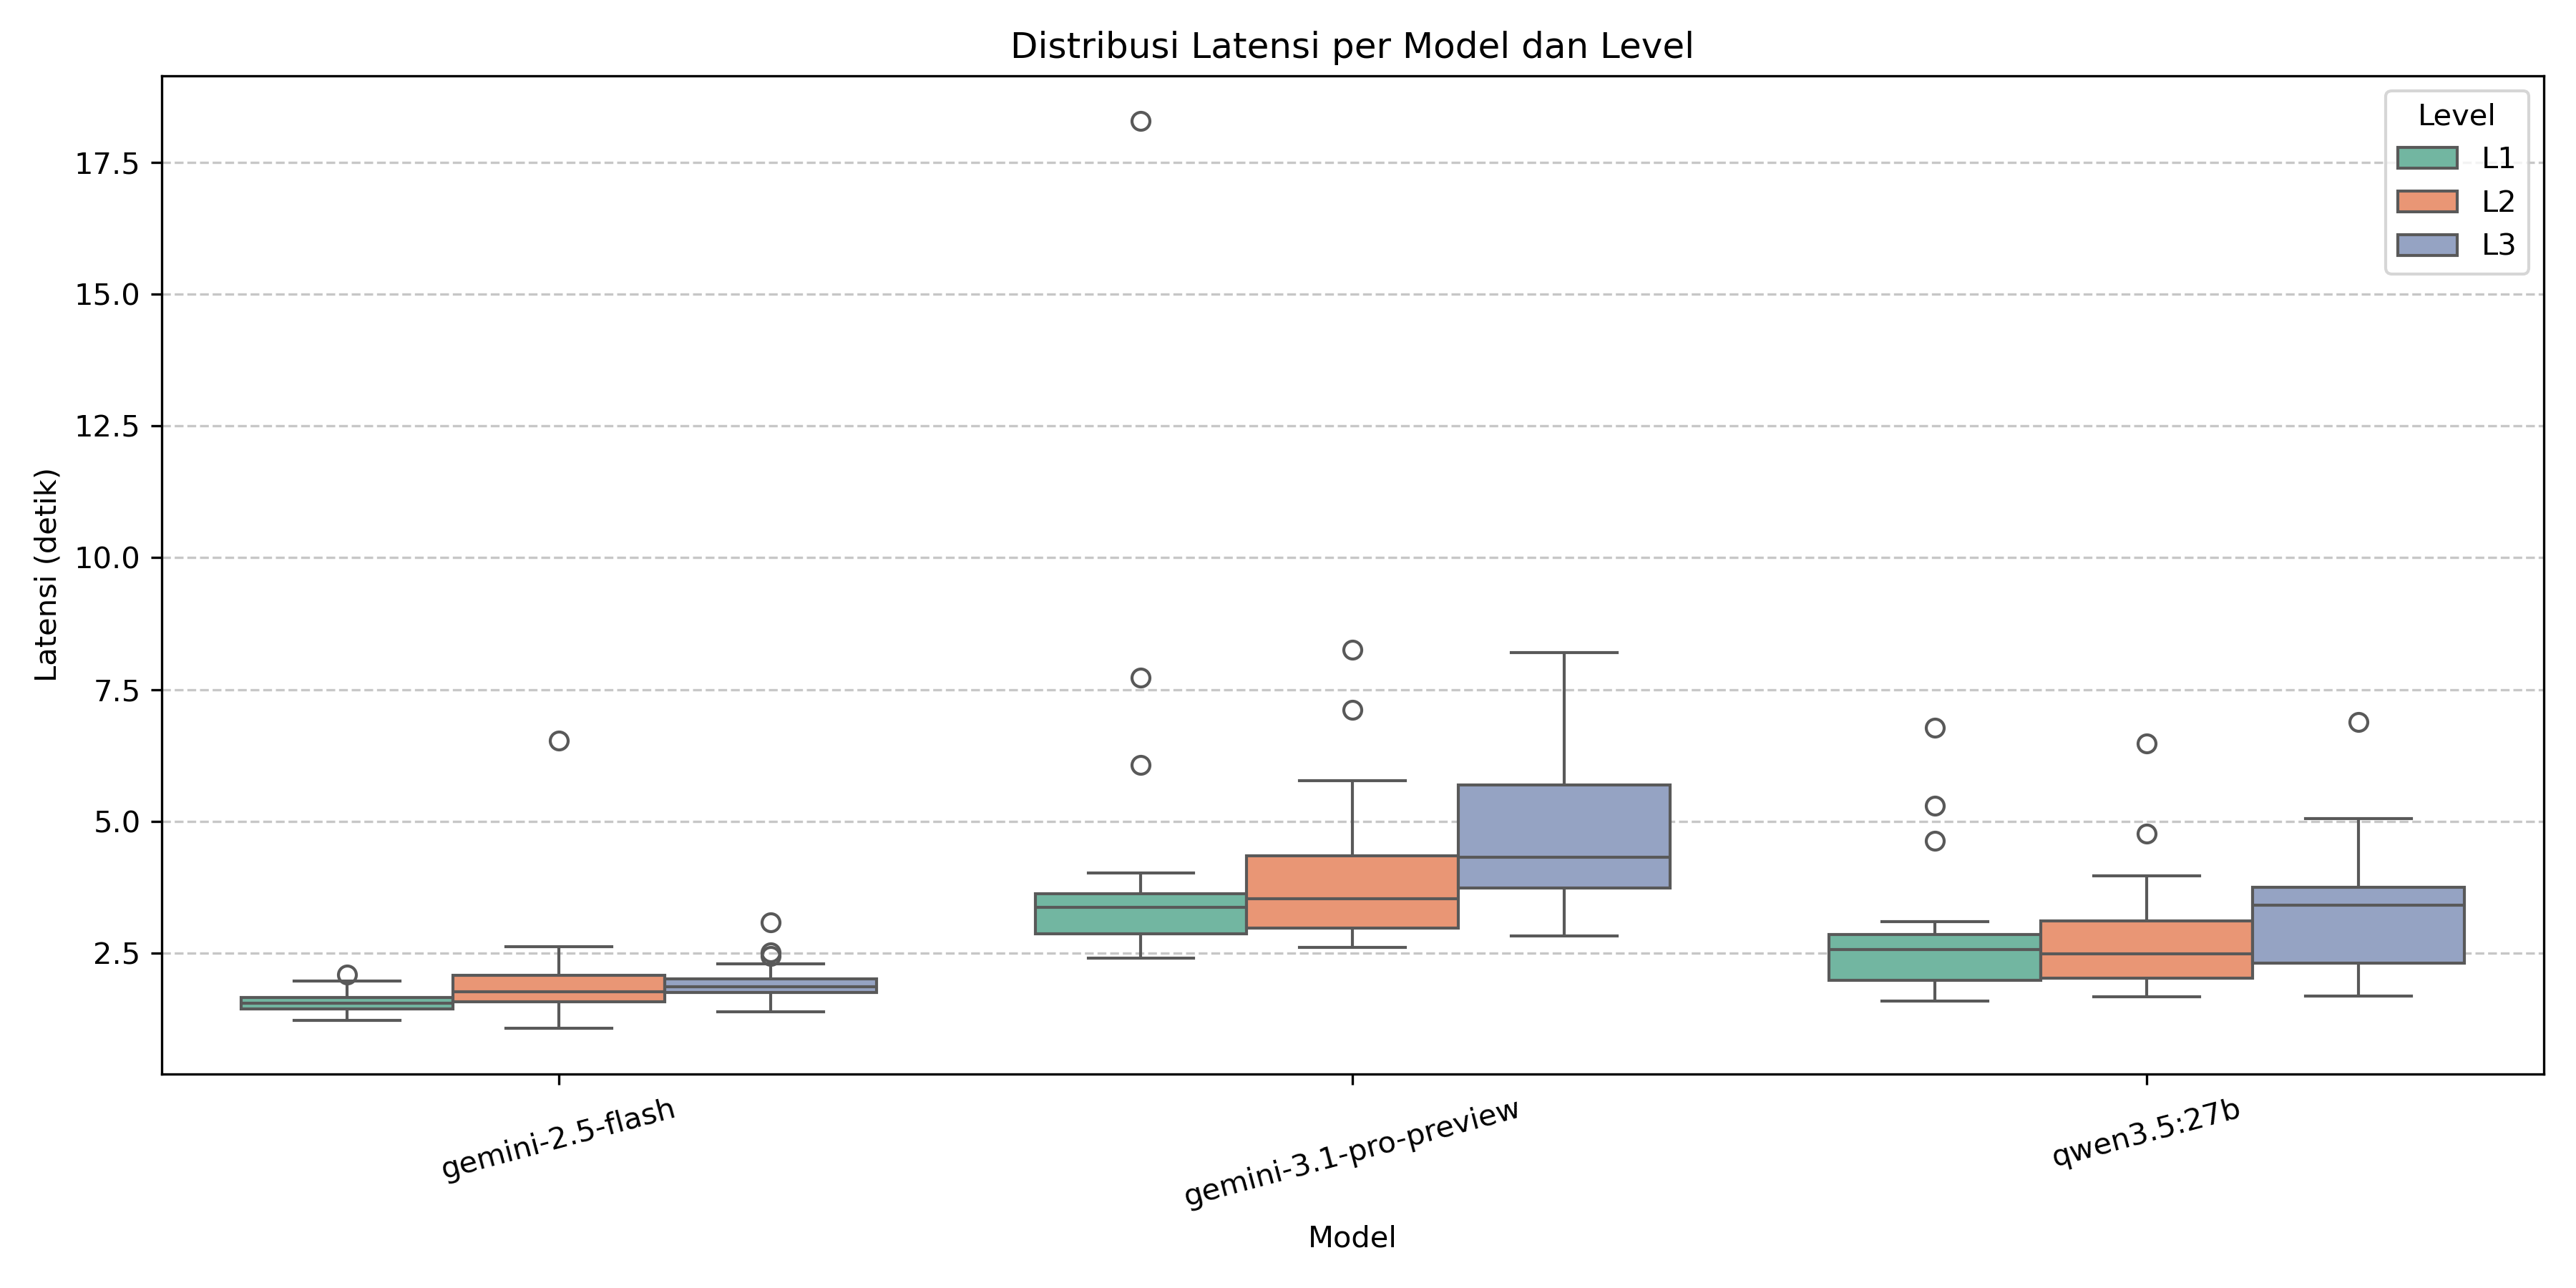
\includegraphics[width=0.8\textwidth]{Init/gambar/boxplots/boxplot_tools_latensi.png}
    \caption{Distribusi Latensi Pengujian Pemanggilan \textit{Tools} per Model}
    \label{fig:boxplot_tools_latensi}
\footnotesize \textbf{Sumber:} Dokumentasi Penulis
\end{figure}

\begin{figure}[H]
    \centering
    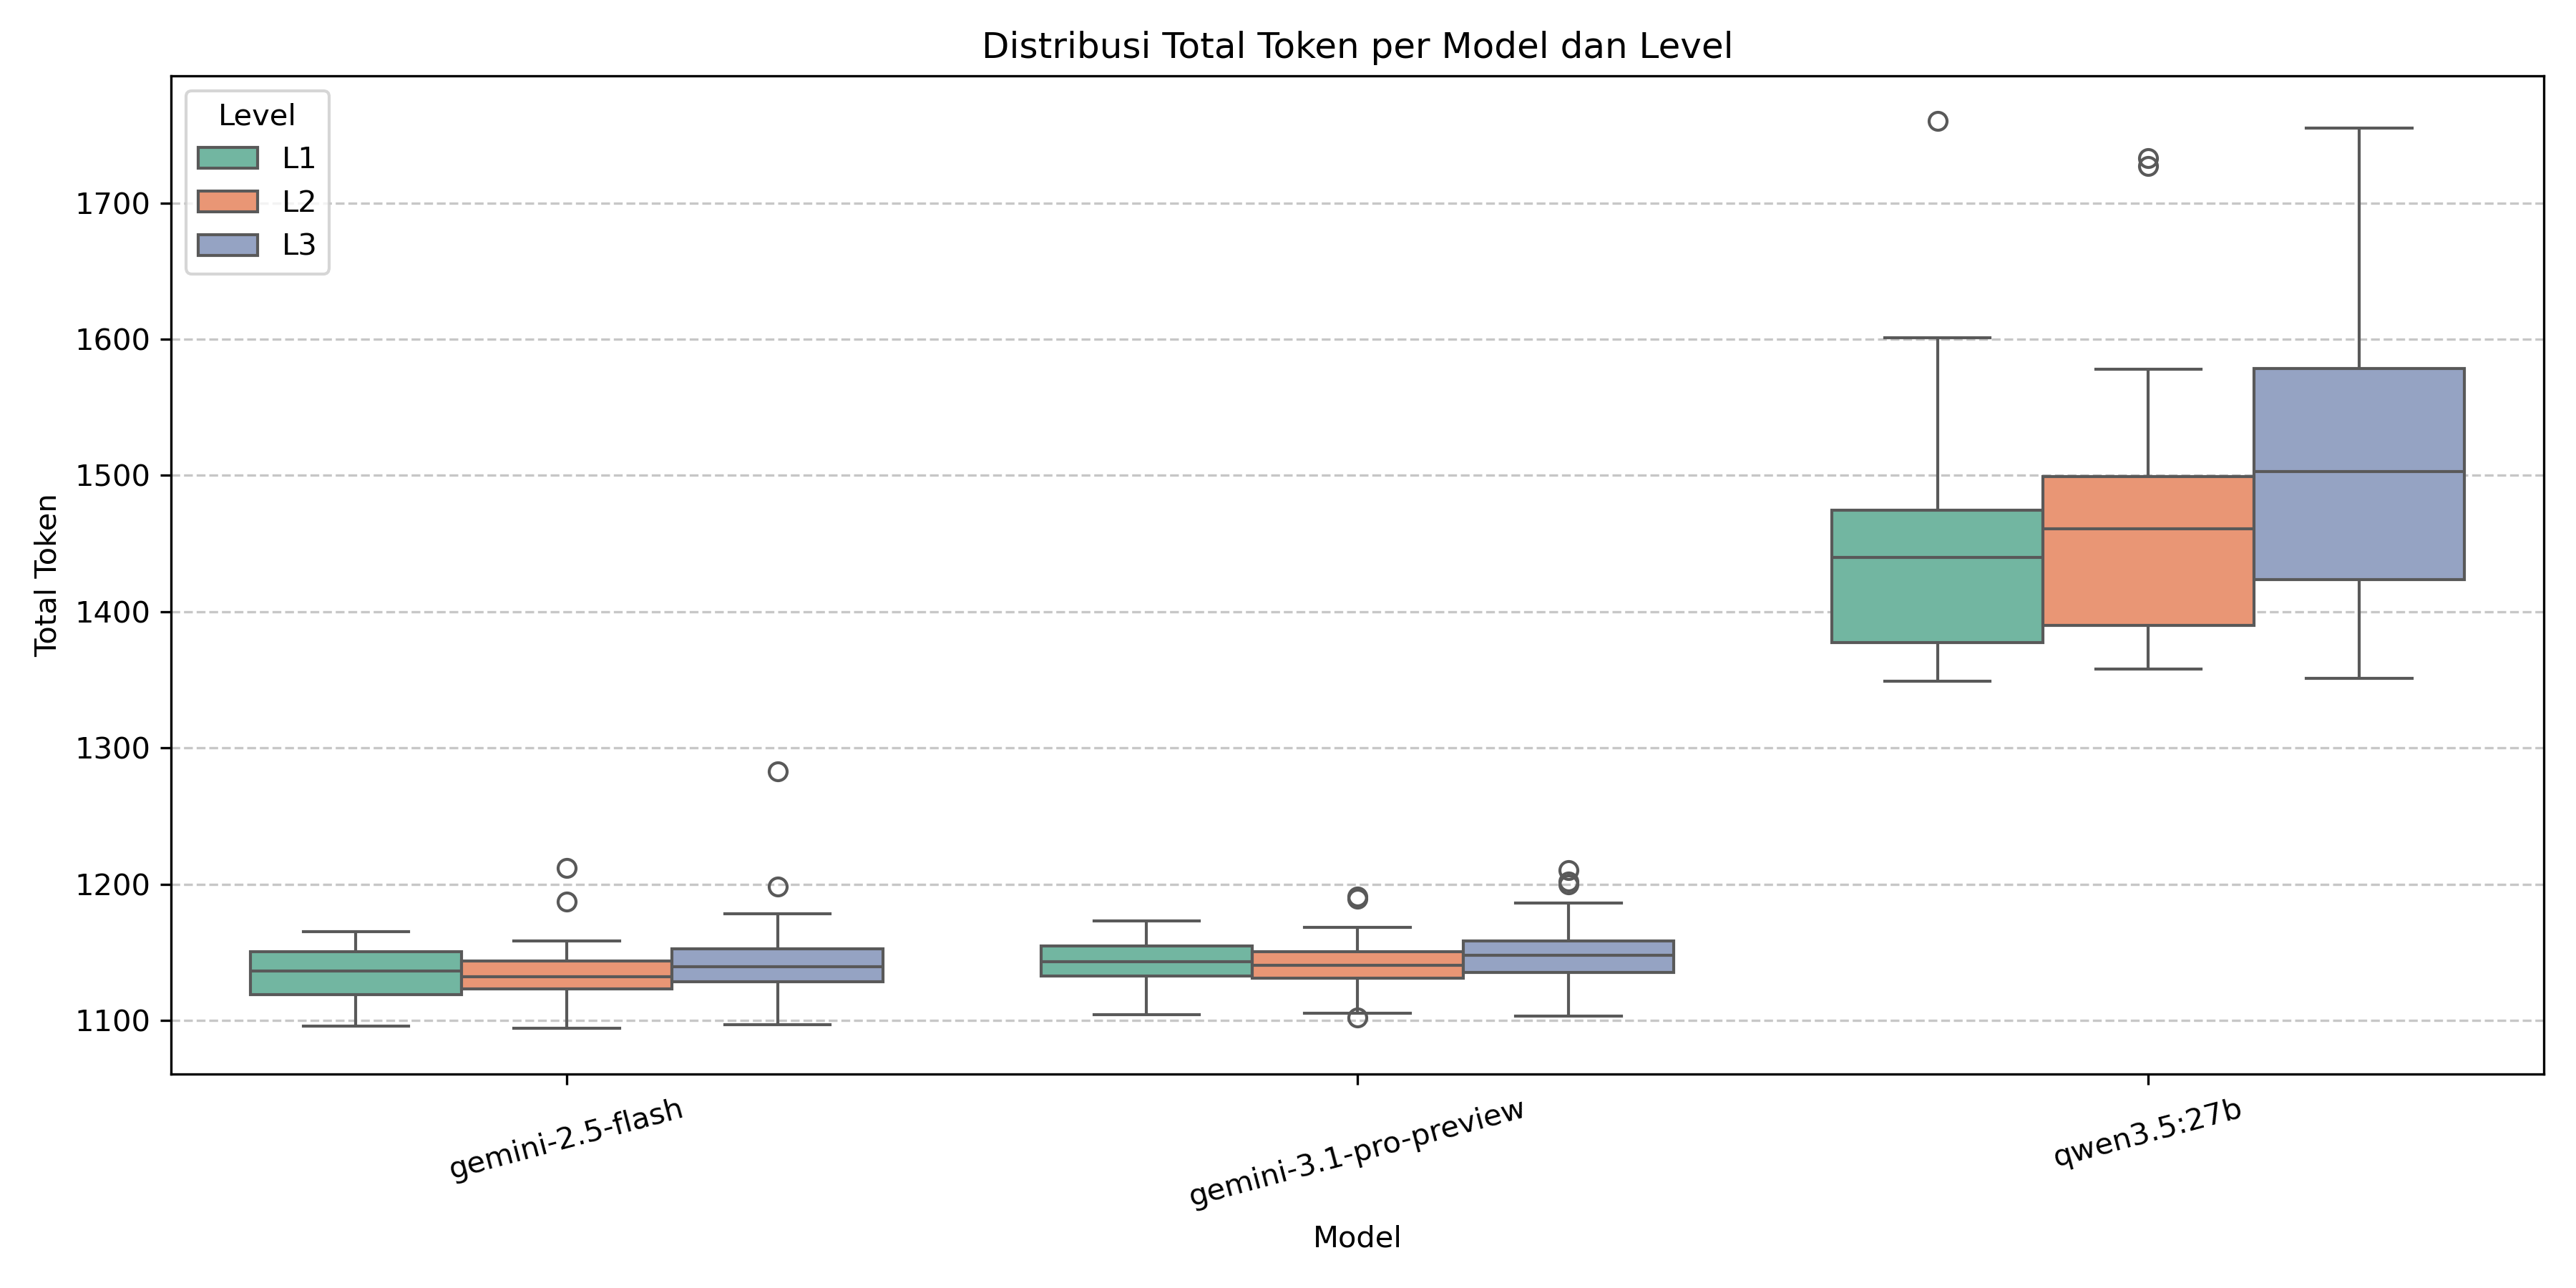
\includegraphics[width=0.8\textwidth]{Init/gambar/boxplots/boxplot_tools_token.png}
    \caption{Distribusi Konsumsi Token Pengujian Pemanggilan \textit{Tools} per Model}
    \label{fig:boxplot_tools_token}
\footnotesize \textbf{Sumber:} Dokumentasi Penulis
\end{figure}

\subsection{Analisis Data Keberhasilan}
Berdasarkan hasil pengujian pada Tabel \ref{tab:tools_summary} dan Tabel \ref{tab:tools_detail}, Gemini 3.1 Pro Preview mencatatkan persentase keberhasilan tertinggi sebesar 98,61\%, diikuti oleh Gemini 2.5 Flash sebesar 93,06\%, dan Qwen 3.5 27B sebesar 88,89\%. Ketiga model menunjukkan performa sempurna pada Level 1 dan Level 2 untuk mayoritas \textit{tools}, dengan seluruh kegagalan terkonsentrasi pada Level 3. Pola ini menunjukkan bahwa ketiga model telah menguasai pemetaan instruksi eksplisit ke \textit{function calling} dengan baik, namun menghadapi tantangan yang berbeda-beda saat instruksi memerlukan penalaran kontekstual yang tinggi. Tiga \textit{tool} yang menjadi sumber kegagalan utama pada Level 3 adalah look\_up\_down, say\_hello, dan toggle\_sit\_stand. Ketiganya memiliki kesamaan karakteristik, yaitu instruksi Level 3 yang diberikan tidak menyebutkan aksi robot secara langsung melainkan mendeskripsikan situasi atau konteks yang mengharuskan model menyimpulkan tindakan yang tepat secara mandiri.

Berdasarkan hasil pengujian, beberapa pola kegagalan pemanggilan \textit{tool} berhasil diidentifikasi. Pada pengujian Gemini 2.5 Flash terhadap \textit{tool} look\_up\_down serta Qwen 3.5 terhadap \textit{tool} say\_hello, model mampu memahami konteks yang diberikan pengguna, namun tidak melakukan pemanggilan \textit{tool}. Model lebih memilih memberikan konfirmasi atau menjelaskan tindakan yang akan dilakukan daripada langsung mengeksekusi \textit{tool}. Pola ini menunjukkan adanya kecenderungan model untuk meminta konfirmasi meskipun konteks yang diberikan telah cukup untuk menentukan aksi yang sesuai. Pada pengujian Gemini 2.5 Flash dan Qwen 3.5 terhadap \textit{tool} toggle\_sit\_stand, model bahkan gagal mengenali maksud instruksi sebagai perintah untuk mengubah postur robot, sehingga respons yang dihasilkan tidak mengarah pada pemanggilan \textit{tool} maupun aksi yang sesuai. Hal ini menunjukkan bahwa model belum mampu menghubungkan makna instruksi dengan \textit{tool} yang tersedia. Model hanya memahami makna literal dari kalimat, tetapi gagal mengidentifikasi bahwa percakapan tersebut merupakan perintah yang seharusnya memicu perubahan postur robot. Karakteristik kegagalan yang berbeda ditemukan pada pengujian Gemini 3.1 Pro dan Qwen 3.5 terhadap \textit{tool} look\_up\_down, serta Qwen 3.5 terhadap \textit{tool} capture\_and\_inspect\_image. Pada kasus ini, model cenderung melakukan \textit{planning} berlebihan sebelum menjalankan \textit{tool}. Alih-alih langsung mengeksekusi \textit{tool} yang diperlukan, model terlebih dahulu berusaha melengkapi informasi lain yang berkaitan dengan proses inspeksi. Akibatnya, pemanggilan \textit{tool} yang sebenarnya sudah dapat dilakukan berdasarkan konteks yang tersedia menjadi tidak dilakukan. Sementara itu, pada pengujian Qwen 3.5 terhadap \textit{tool} async\_move, ditemukan kesalahan dalam pemilihan \textit{tool}. Model memilih \textit{tool} yang memiliki fungsi berbeda dengan aksi yang dimaksud oleh pengguna. Hal ini menunjukkan adanya kegagalan dalam memetakan makna bahasa alami ke fungsi \textit{tool} yang sesuai.

Secara keseluruhan, analisis ini membuktikan bahwa instruksi yang bersifat abstrak dan multi-interpretasi pada Level 3 merupakan tantangan utama bagi agen MLLM. Model dengan ukuran parameter besar seperti Gemini 3.1 Pro mampu menalar konteks spasial dan situasional dengan lebih baik, meskipun sempat gagal karena melakukan \textit{planning} berlebihan. Di sisi lain, model yang lebih kecil atau dioptimasi untuk kecepatan, seperti Gemini 2.5 Flash dan Qwen 3.5 27B, cenderung lebih rentan terhadap kegagalan dalam penalaran intruksi abstrak, Baik dalam bentuk kegagalan memicu tool, sehingga model hanya memberikan respons tekstual, maupun kesalahan dalam pemilihan tool yang tepat.


\subsection{Analisis Latensi dan Konsumsi \textit{Token}}
Berdasarkan distribusi latensi (Gambar \ref{fig:boxplot_tools_latensi}) dan konsumsi token (Gambar \ref{fig:boxplot_tools_token}), terlihat tren yang konsisten terhadap kompleksitas level instruksi dan karakteristik model. Secara umum, Gemini 2.5 Flash memiliki waktu respons paling singkat pada seluruh level pengujian, menunjukkan performa yang lebih baik dari sisi latensi dibandingkan model lainnya. Qwen 3.5 berada di posisi menengah, sementara Gemini 3.1 Pro mencatatkan latensi tertinggi akibat kecenderungannya melakukan proses penalaran yang lebih kompleks. Peningkatan latensi yang sejalan dengan naiknya level kesulitan instruksi menunjukkan bahwa kompleksitas \textit{prompt} berdampak langsung pada waktu pemrosesan model. Dari sisi konsumsi token, kedua varian Gemini memiliki penggunaan yang stabil dan identik di seluruh level karena berbagi arsitektur \textit{tokenizer} yang sama. Sebaliknya, Qwen 3.5 mengonsumsi token jauh lebih besar dengan rentang yang lebar akibat model ini sering memberikan respons tekstual yang panjang. Temuan ini membuktikan bahwa jumlah token tidak selalu berbanding lurus dengan waktu respons, tingginya latensi Gemini 3.1 Pro bersumber dari mekanisme penalaran internal (\textit{reasoning}), bukan sekadar panjang keluaran.

% =============================================================================
% PENGUJIAN 2: ANALISIS OBJEK
% =============================================================================
\section{Pengujian Analisis Objek}
\label{sec:pengujian_inspeksi}
Pengujian ini bertujuan untuk mengevaluasi kemampuan model MLLM dalam menganalisis kondisi fisik objek inspeksi melalui \textit{image} yang ditangkap oleh kamera robot. Evaluasi dilakukan dengan membandingkan hasil analisis model terhadap kondisi aktual objek berdasarkan dokumen \textit{Standard Operating Procedure} yang relevan.

\subsection{Skenario Pengujian}
Pengujian dilakukan terhadap tiga jenis objek target inspeksi, yaitu APAR, stop kontak, dan tong sampah. Setiap objek diuji dalam tiga kondisi yang berbeda sebagai berikut:

\begin{table}[H]
\centering
\caption{Skenario Kondisi Pengujian Analisis Objek (APAR dan Stop Kontak)}
\label{tab:skenario_analisis_objek_1}
\renewcommand{\arraystretch}{1.5}
\resizebox{\linewidth}{!}{
\begin{tabular}{|l|l|p{5cm}|c|}
\hline
\textbf{Objek} & \textbf{Tipe Kondisi} & \textbf{Deskripsi} & \textbf{Contoh \textit{Image}} \\
\hline
\multirow{3}{*}{APAR} & Normal & APAR terpasang sesuai prosedur & 
\begin{minipage}{3.5cm} \vspace{2mm} \centering 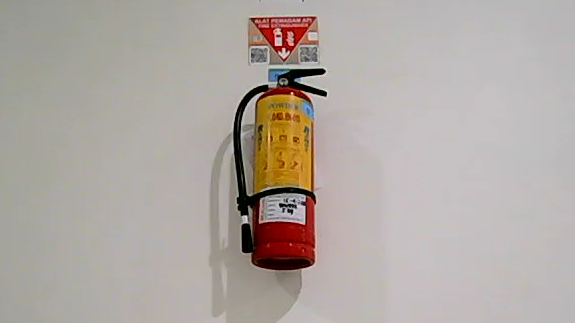
\includegraphics[height=2cm]{Init/gambar/image_uji/apar/normal/1781265608506.png} \vspace{2mm} \end{minipage} \\
\cline{2-4}
& Anomali 1 & APAR tergeletak di lantai & 
\begin{minipage}{3.5cm} \vspace{2mm} \centering 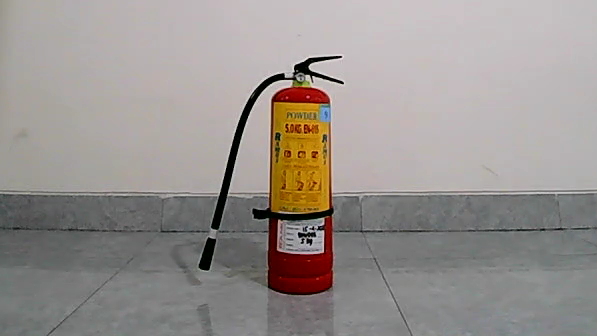
\includegraphics[height=2cm]{Init/gambar/image_uji/apar/tergeletak/1781265760647.png} \vspace{2mm} \end{minipage} \\
\cline{2-4}
& Anomali 2 & Selang tidak menempel pada klip \textit{body} & 
\begin{minipage}{3.5cm} \vspace{2mm} \centering 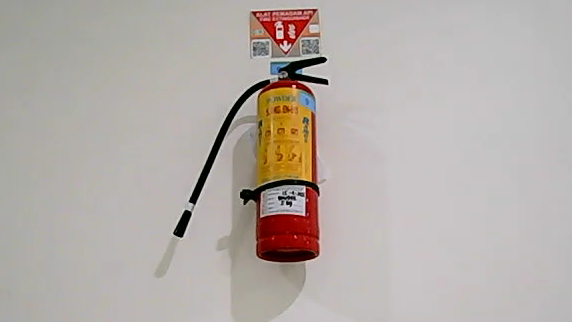
\includegraphics[height=2cm]{Init/gambar/image_uji/apar/selang_lepas/1781265701773.png} \vspace{2mm} \end{minipage} \\
\hline
\multirow{3}{*}{Stop Kontak} & Normal & Stop kontak dalam kondisi baik & 
\begin{minipage}{3.5cm} \vspace{2mm} \centering 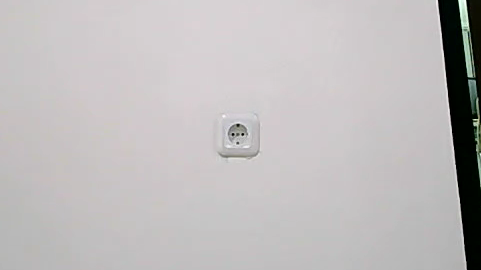
\includegraphics[height=2cm]{Init/gambar/image_uji/stop_kontak/normal/1781266626664.png} \vspace{2mm} \end{minipage} \\
\cline{2-4}
& Kondisi 1 & Terdapat steker normal yang terpasang & 
\begin{minipage}{3.5cm} \vspace{2mm} \centering 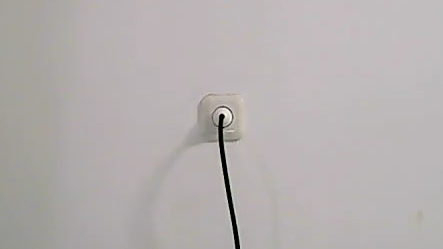
\includegraphics[height=2cm]{Init/gambar/image_uji/stop_kontak/tercolok_steker/1781266432749.png} \vspace{2mm} \end{minipage} \\
\cline{2-4}
& Anomali & Steker dengan kabel putus/rusak & 
\begin{minipage}{3.5cm} \vspace{2mm} \centering 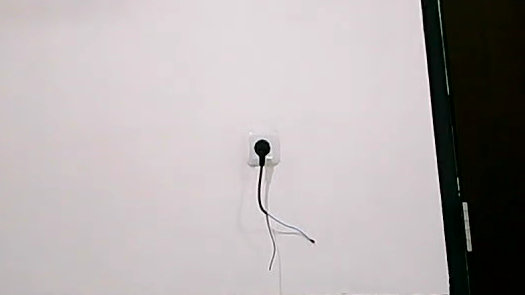
\includegraphics[height=2cm]{Init/gambar/image_uji/stop_kontak/steker_rusak/1781266701947.png} \vspace{2mm} \end{minipage} \\
\hline
\end{tabular}
}
\end{table}

\begin{table}[H]
\centering
\caption{Skenario Kondisi Pengujian Analisis Objek (Tong Sampah)}
\label{tab:skenario_analisis_objek_2}
\renewcommand{\arraystretch}{1.5}
\resizebox{\linewidth}{!}{
\begin{tabular}{|l|l|p{5cm}|c|}
\hline
\textbf{Objek} & \textbf{Tipe Kondisi} & \textbf{Deskripsi} & \textbf{Contoh Gambar} \\
\hline
\multirow{3}{*}{Tong Sampah} & Normal & Tiga tong sampah tersusun rapi & 
\begin{minipage}{3.5cm} \vspace{2mm} \centering 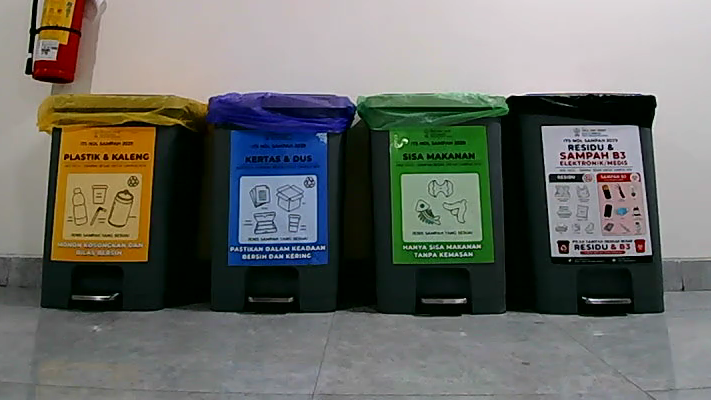
\includegraphics[height=2cm]{Init/gambar/image_uji/tong_sampah/normal/1781265874120.png} \vspace{2mm} \end{minipage} \\
\cline{2-4}
& Anomali 1 & Hanya terdapat dua tong sampah (tidak lengkap) & 
\begin{minipage}{3.5cm} \vspace{2mm} \centering 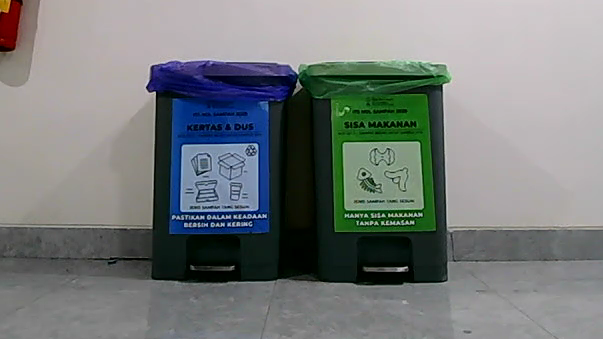
\includegraphics[height=2cm]{Init/gambar/image_uji/tong_sampah/tong_kurang/1781265905093.png} \vspace{2mm} \end{minipage} \\
\cline{2-4}
& Anomali 2 & Tong sampah berantakan dengan sampah berserakan & 
\begin{minipage}{3.5cm} \vspace{2mm} \centering 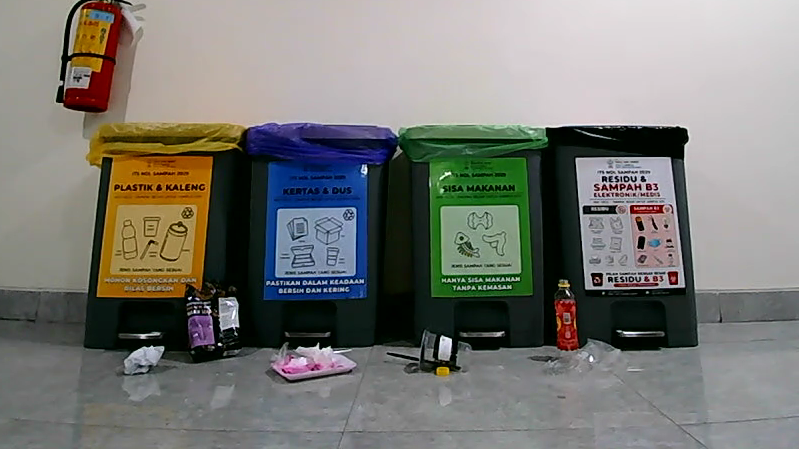
\includegraphics[height=2cm]{Init/gambar/image_uji/tong_sampah/sampah_berserakan/1781266320437.png} \vspace{2mm} \end{minipage} \\
\hline
\end{tabular}
}
\end{table}

Setiap kondisi diuji sebanyak tiga kali dari sudut pengambilan \textit{image} yang berbeda-beda untuk menguji konsistensi analisis model terhadap variasi sudut pandang kamera robot. Total terdapat $3 \times 3 \times 3 = 27$ kasus uji per model.

\subsection{Hasil Pengujian}

\begin{table}[H]
\centering
\caption{Ringkasan Hasil Pengujian Analisis Objek}
\label{tab:inspect_summary}
\begin{tabular}{|l|c|c|c|}
\hline
\textbf{Metrik} & \textbf{Gemini 2.5 Flash} & \textbf{Gemini 3.1 Pro} & \textbf{Qwen 3.5 27B} \\
\hline
Persentase Keberhasilan & 85,19\% & 100,00\% & 85,19\% \\
\hline
Rata-rata Latensi (detik) & 9,62 & 19,31 & 35,29 \\
\hline
Rata-rata Total Token & 1.980 & 3.297 & 5.071 \\
\hline
\end{tabular}
\end{table}

% --- Tabel Detail Per Objek Per Kondisi ---
\begin{longtable}{|l|l|c|c|c|c|c|c|}
\caption{Detail Hasil Pengujian Analisis Objek per Kondisi} \label{tab:inspect_detail} \\
\hline
\multirow{2}{*}{\textbf{Objek}} & \multirow{2}{*}{\textbf{Kondisi}} & \multicolumn{2}{c|}{\textbf{Gemini 2.5 Flash}} & \multicolumn{2}{c|}{\textbf{Gemini 3.1 Pro}} & \multicolumn{2}{c|}{\textbf{Qwen 3.5 27B}} \\
\cline{3-8}
& & \textbf{Skor} & \textbf{Latensi} & \textbf{Skor} & \textbf{Latensi} & \textbf{Skor} & \textbf{Latensi} \\
\hline
\endfirsthead
\hline
\multirow{2}{*}{\textbf{Objek}} & \multirow{2}{*}{\textbf{Kondisi}} & \multicolumn{2}{c|}{\textbf{Gemini 2.5 Flash}} & \multicolumn{2}{c|}{\textbf{Gemini 3.1 Pro}} & \multicolumn{2}{c|}{\textbf{Qwen 3.5 27B}} \\
\cline{3-8}
& & \textbf{Skor} & \textbf{Latensi} & \textbf{Skor} & \textbf{Latensi} & \textbf{Skor} & \textbf{Latensi} \\
\hline
\endhead
APAR & Tergeletak di lantai & 3/3 & 8,88 & 3/3 & 19,91 & 3/3 & 36,64 \\
\hline
APAR & Selang tidak menempel & 0/3 & 8,22 & 3/3 & 20,32 & 1/3 & 47,83 \\
\hline
APAR & Normal & 3/3 & 11,38 & 3/3 & 21,68 & 2/3 & 38,34 \\
\hline
Stop Kontak & Steker kabel putus & 2/3 & 9,02 & 3/3 & 17,68 & 2/3 & 27,13 \\
\hline
Stop Kontak & Normal & 3/3 & 7,82 & 3/3 & 15,32 & 3/3 & 23,43 \\
\hline
Stop Kontak & Steker normal & 3/3 & 8,98 & 3/3 & 15,45 & 3/3 & 32,98 \\
\hline
Tong Sampah & Hanya dua tong & 3/3 & 9,35 & 3/3 & 19,51 & 3/3 & 36,94 \\
\hline
Tong Sampah & Normal & 3/3 & 11,31 & 3/3 & 22,72 & 3/3 & 41,96 \\
\hline
Tong Sampah & Sampah berserakan & 3/3 & 11,65 & 3/3 & 21,19 & 3/3 & 32,38 \\
\hline
\end{longtable}

\begin{figure}[H]
    \centering
    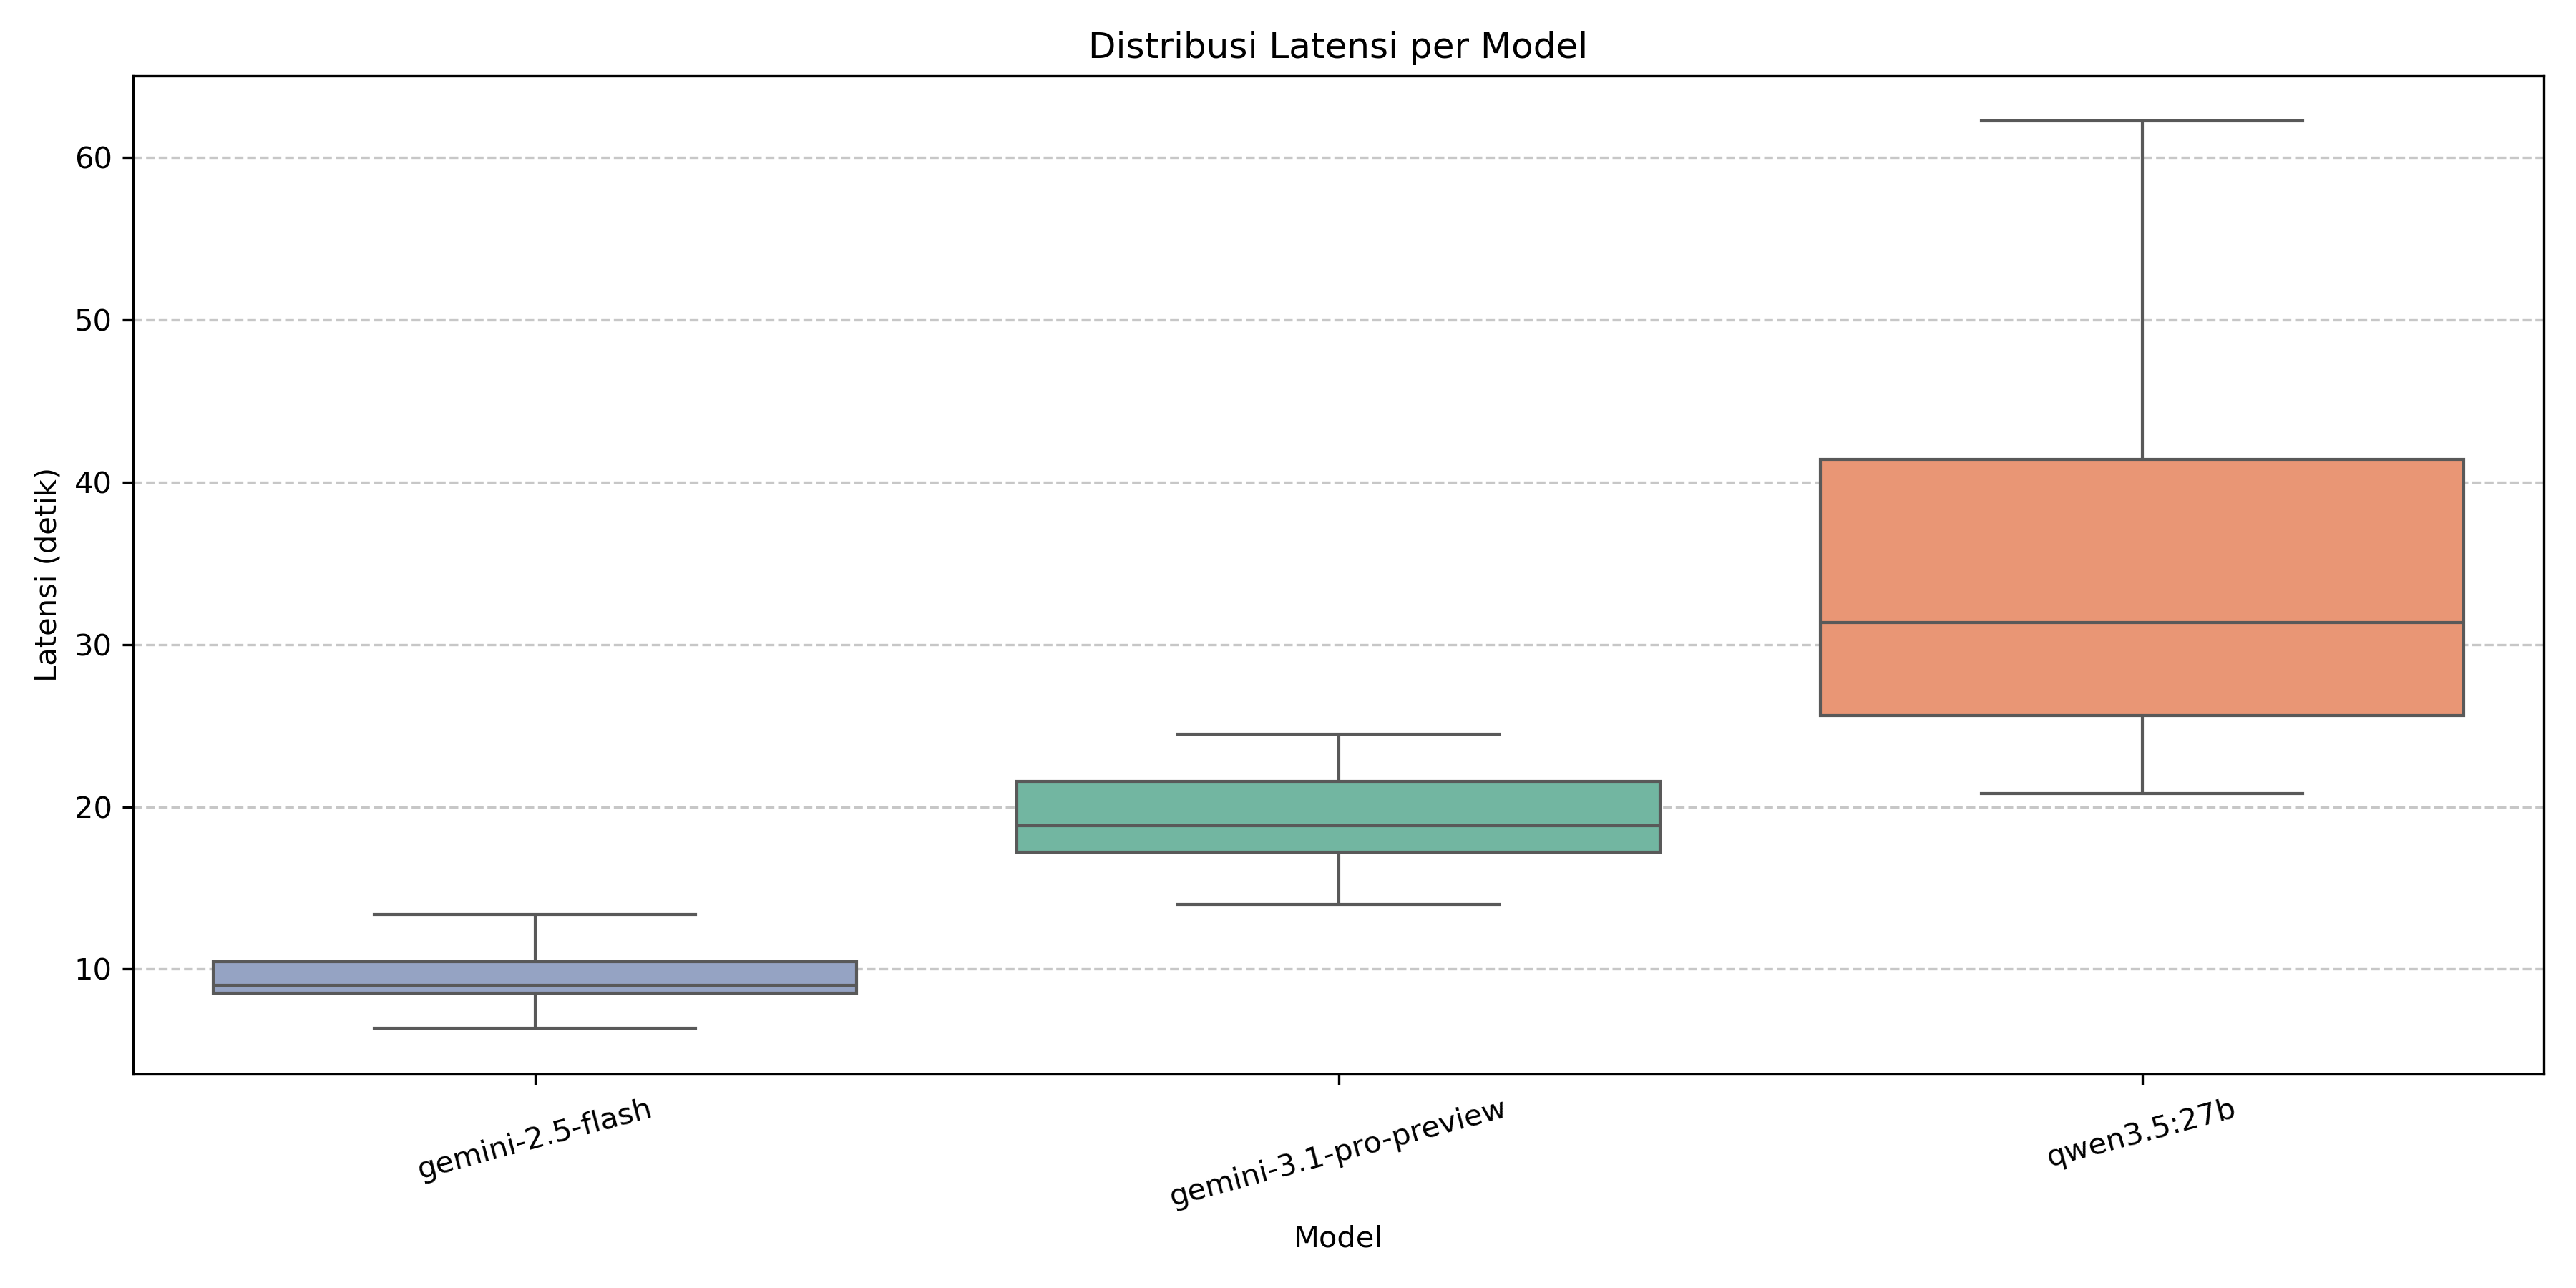
\includegraphics[width=0.8\textwidth]{Init/gambar/boxplots/boxplot_inspeksi_latensi.png}
    \caption{Distribusi Latensi Pengujian Analisis Objek per Model}
    \label{fig:boxplot_inspeksi_latensi}
\footnotesize \textbf{Sumber:} Dokumentasi Penulis
\end{figure}

\begin{figure}[H]
    \centering
    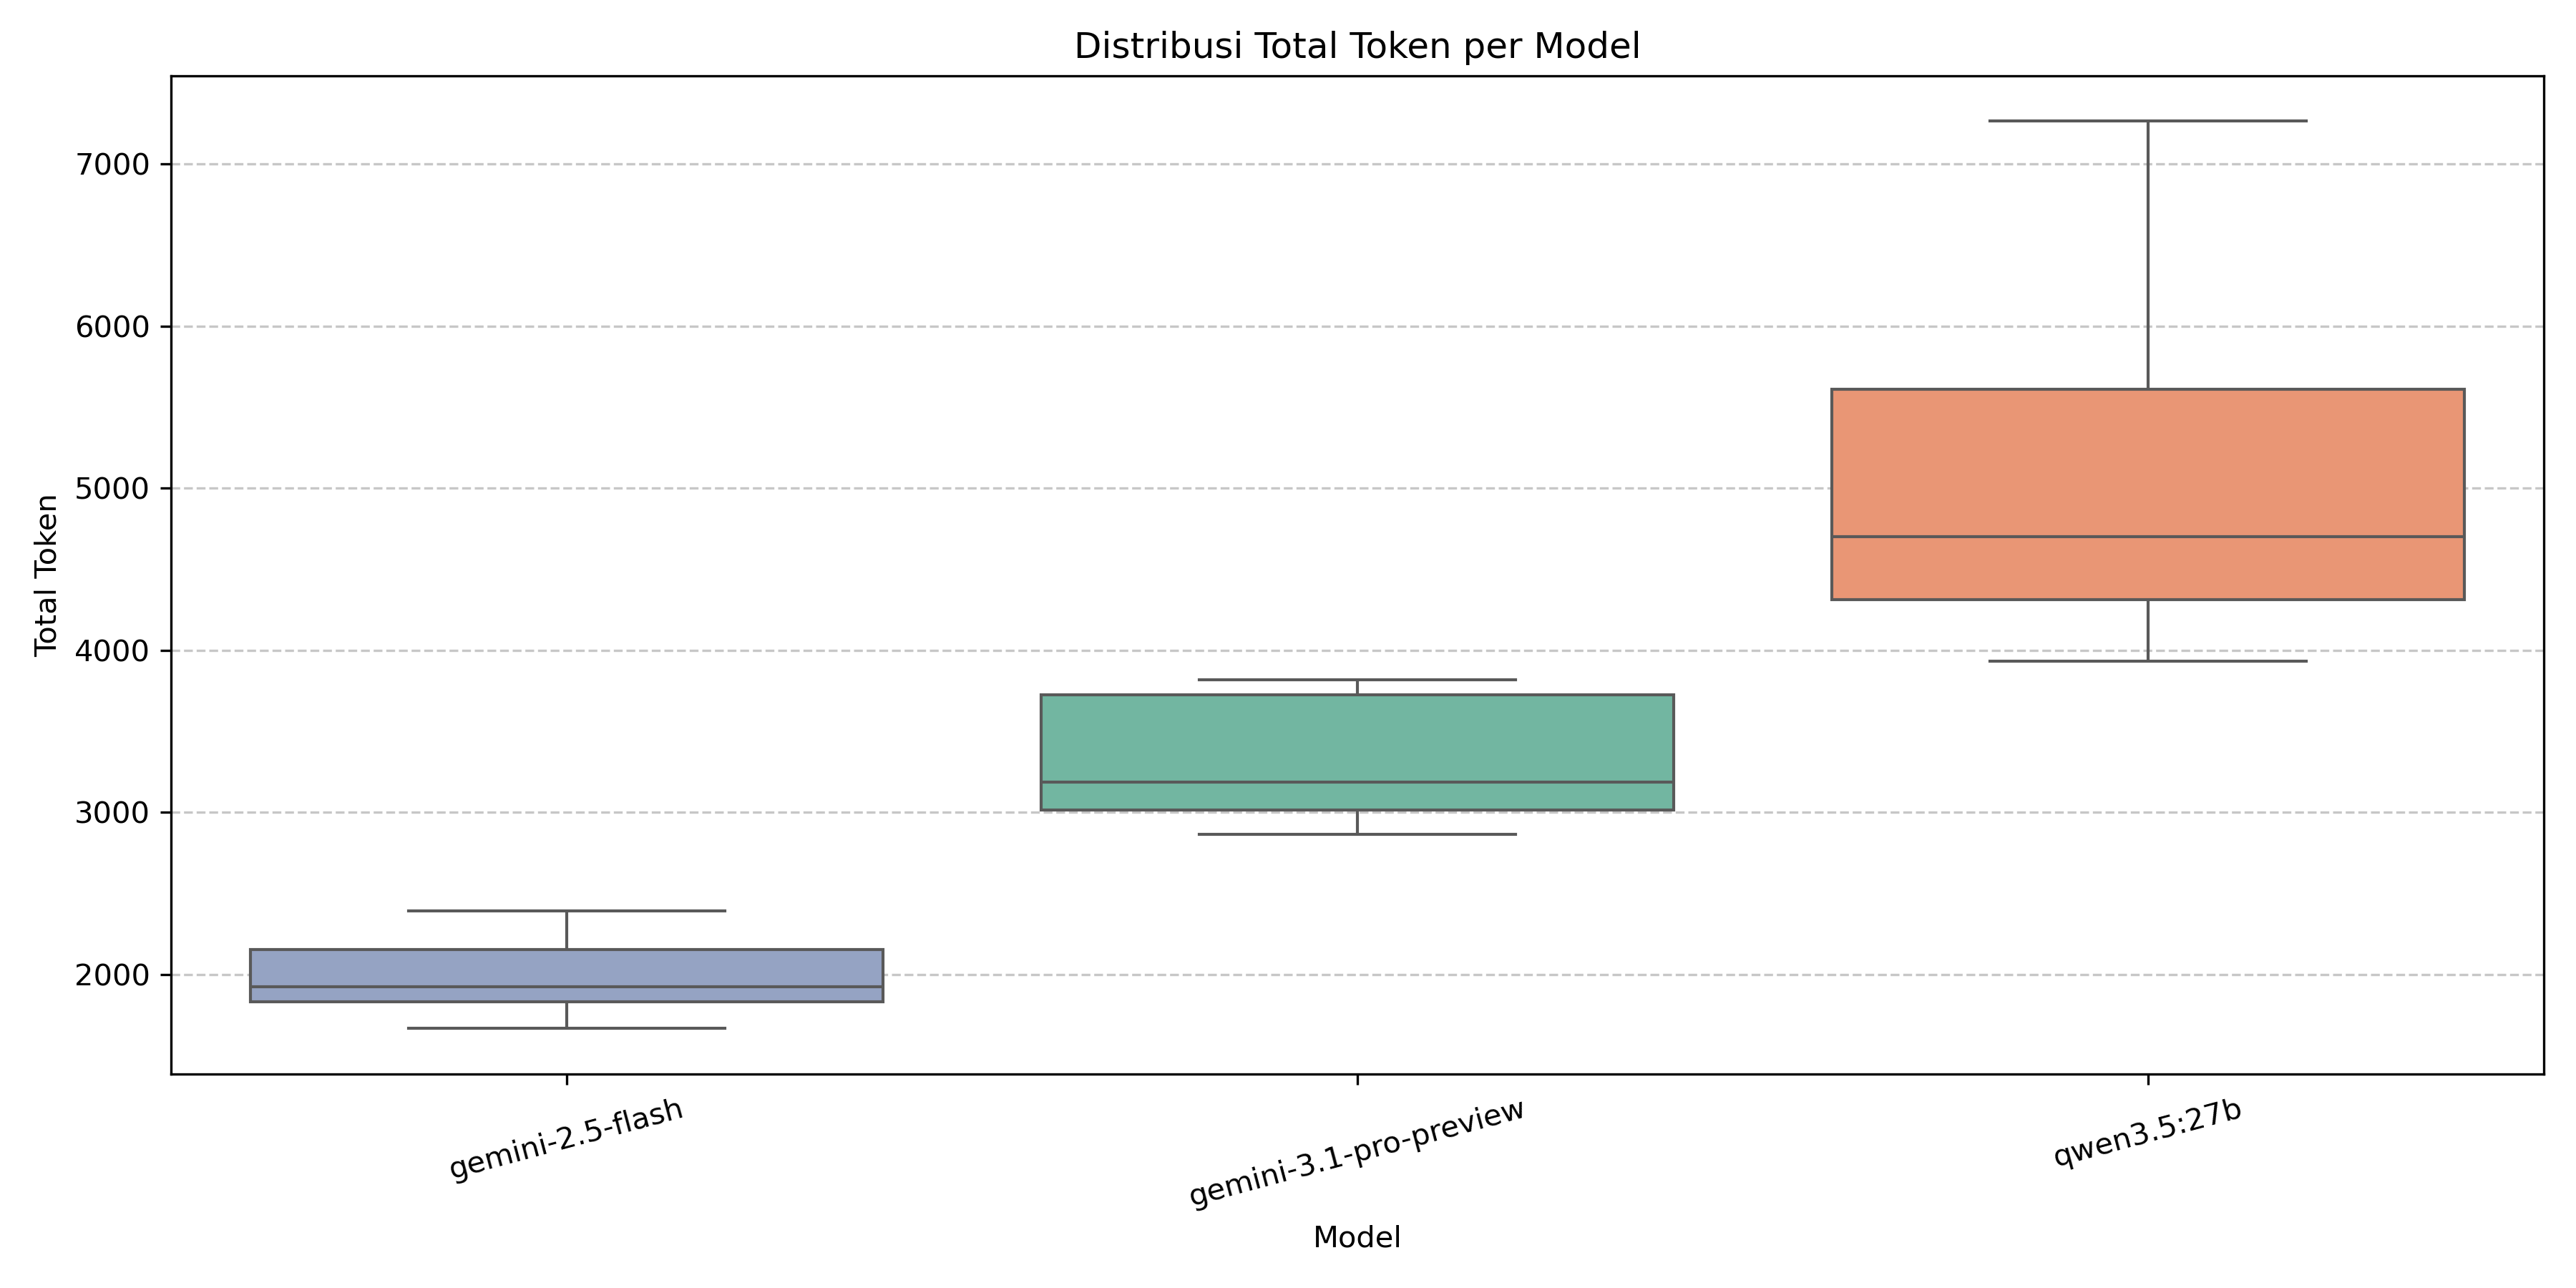
\includegraphics[width=0.8\textwidth]{Init/gambar/boxplots/boxplot_inspeksi_token.png}
    \caption{Distribusi Konsumsi Token Pengujian Analisis Objek per Model}
    \label{fig:boxplot_inspeksi_token}
\footnotesize \textbf{Sumber:} Dokumentasi Penulis
\end{figure}


\subsection{Analisis Data Keberhasilan}
Berdasarkan hasil pengujian pada Tabel \ref{tab:inspect_summary} dan Tabel \ref{tab:inspect_detail}, terlihat perbedaan performa yang signifikan antara model kelas atas dengan model yang lebih ringan dalam tugas analisis visual berbasis \textit{Multimodal Large Language Model} (MLLM). Gemini 3.1 Pro Preview mencatatkan performa sempurna dengan tingkat keberhasilan 100\% untuk seluruh kasus uji di berbagai variasi objek, kondisi, dan sudut pengambilan \textit{image}. Sebaliknya, Gemini 2.5 Flash dan Qwen 3.5 27B sama-sama mencatatkan tingkat keberhasilan 85,19\%. Meskipun tingkat kegagalan kedua model ini identik secara kuantitatif, analisis kualitatif terhadap respons model menunjukkan pola kegagalan yang berbeda.

Kasus ``selang APAR tidak menempel pada klip \textit{body}'' terbukti menjadi skenario paling menantang. Gemini 2.5 Flash mengalami kegagalan pada kondisi ini, di mana model berhalusinasi dengan menyatakan bahwa selang terpasang dengan baik. Qwen 3.5 juga mengalami kesulitan serupa karena memberikan hasil yang keliru terkait posisi ujung selang. Kegagalan pada skenario ini mengindikasikan kelemahan pada Flash dan Qwen dalam memahami detail spasial dan hubungan struktural antar komponen objek dari sebuah \textit{image}, tugas yang berhasil diselesaikan dengan baik oleh kapabilitas penalaran spasial Gemini 3.1 Pro.

Selain masalah penalaran spasial kompleks, Qwen 3.5 juga menunjukkan kelemahan pada tugas deteksi warna. Pada pengujian APAR dengan kondisi normal, Qwen 3.5 sempat gagal karena salah mengidentifikasi warna dominan tabung. Kesalahan deteksi ini berakar dari kondisi fisik APAR yang ditutupi oleh stiker label berwarna kuning pada sebagian besar tabungnya. Meskipun SOP secara eksplisit telah memberikan instruksi untuk mengabaikan warna label stiker, Qwen 3.5 terdistraksi oleh dominasi piksel kuning dan gagal mematuhi instruksi pengecualian tersebut. Kesalahan interpretasi warna semacam ini menjadi indikasi awal bahwa arsitektur \textit{Multimodal Large Language Model} pada dasarnya masih rentan terhadap jebakan visual mayoritas akibat dominasi warna tertentu, sebuah kerentanan komputasi visual yang bersifat stokastik dan berpotensi muncul pada model kelas atas sekalipun.

Kegagalan lain yang dialami oleh Flash dan Qwen terjadi pada skenario stop kontak dengan anomali steker putus atau rusak, di mana kedua model mengalami kesalahan \textit{false negative} dengan menyatakan kondisi steker aman dan utuh. Kegagalan ini menyoroti batasan resolusi dan kemampuan atensi model yang lebih kecil dalam mendeteksi anomali berskala detail ketika objek tersebut menempati proporsi piksel yang relatif kecil dibandingkan keseluruhan \textit{image}.

\subsection{Analisis Latensi dan Konsumsi \textit{Token}}
Berdasarkan distribusi latensi (Gambar \ref{fig:boxplot_inspeksi_latensi}) dan konsumsi token (Gambar \ref{fig:boxplot_inspeksi_token}), terlihat perubahan tren yang signifikan dibandingkan pengujian pemanggilan \textit{tool} sebelumnya akibat adanya penambahan dimensi multimodal berupa \textit{image}. Gemini 2.5 Flash tetap konsisten menjadi model tercepat dengan rata-rata latensi terendah. Sebaliknya, Qwen 3.5 mengalami pergeseran performa yang signifikan, jika pada pengujian berbasis teks sebelumnya model lokal ini cepat, pada analisis \textit{image} latensinya melonjak drastis menjadi yang terlama. Pembalikan tren ini terjadi karena proses ekstraksi fitur visual, kemungkinan memberi beban komputasi yang besar bagi perangkat keras lokal, melebihi beban pemrosesan instruksi teks murni. Gemini 3.1 Pro menunjukkan latensi yang lebih tinggi dibandingkan Gemini 2.5 Flash, sebanding dengan hasilnya yang mencapai akurasi sempurna pada seluruh skenario pengujian. Dari sisi penggunaan token, tren kesamaan antara kedua varian Gemini tidak lagi terlihat, kemungkinan akibat perbedaan mekanisme konversi \textit{image} ke \textit{image token}, Gemini 2.5 Flash mengonsumsi token paling sedikit berkat \textit{downscaling} resolusi, sedangkan Gemini 3.1 Pro menggunakan jauh lebih banyak demi mengekstrak fitur \textit{image} beresolusi tinggi. Sementara itu, Qwen 3.5 tetap konsisten menjadi model yang paling boros akibat inefisiensi arsitektur \textit{vision encoder} dan kecenderungannya memberikan penjelasan yang terlalu deskriptif.



% =============================================================================
% PENGUJIAN 3: PEMBUATAN PLAN
% =============================================================================
\section{Pengujian Pembuatan \textit{Plan} Inspeksi}
\label{sec:pengujian_plan}

\subsection{Tujuan Pengujian}
Pengujian ini bertujuan untuk mengevaluasi kemampuan model MLLM dalam menyusun rencana inspeksi yang optimal berdasarkan instruksi operator. Evaluasi mencakup kebenaran dalam mengidentifikasi objek target dari basis data, ketepatan urutan kunjungan berdasarkan efisiensi jarak terpendek dari posisi robot saat ini, serta kemampuan model dalam menolak permintaan yang tidak valid.

\subsection{Skenario Pengujian}
Dataset pengujian terdiri dari 12 kasus uji yang dibagi menjadi empat level kesulitan sebagai berikut:

\begin{enumerate}
    \item \textbf{Level Mudah} (1 objek target): Instruksi untuk menginspeksi satu objek tunggal. Model harus mengidentifikasi objek terdekat dan menyusun rencana sederhana. (3 kasus uji)
    \item \textbf{Level Sedang} (3 objek target): Instruksi untuk menginspeksi tiga objek dari kategori berbeda. Model harus mengurutkan kunjungan berdasarkan jarak terpendek. (3 kasus uji)
    \item \textbf{Level Sulit} (6 objek target): Instruksi untuk menginspeksi enam objek dari berbagai kategori. Model harus menyusun rute efisien untuk kunjungan yang lebih kompleks. (3 kasus uji)
    \item \textbf{Level Mustahil} (objek tidak valid): Instruksi yang meminta inspeksi objek atau lokasi yang tidak terdaftar dalam basis data. Model harus mampu menolak permintaan dan memberikan penjelasan. (3 kasus uji)
\end{enumerate}

Setiap kasus uji menyertakan posisi koordinat robot saat ini sebagai konteks tambahan untuk pengambilan keputusan urutan rute.

\subsection{Hasil Pengujian}

\begin{longtable}{|l|c|c|c|c|c|c|c|c|c|c|}
\caption{Hasil Pengujian Pembuatan \textit{Plan} Inspeksi} \label{tab:plan_results} \\
\hline
\multirow{2}{*}{\textbf{Level}} & \multirow{2}{*}{\textbf{\shortstack{Jumlah\\Objek}}} & \multicolumn{3}{c|}{\textbf{Gemini 2.5 Flash}} & \multicolumn{3}{c|}{\textbf{Gemini 3.1 Pro}} & \multicolumn{3}{c|}{\textbf{Qwen 3.5 27B}} \\
\cline{3-11}
& & \textbf{Skor} & \textbf{Rute} & \textbf{Latensi} & \textbf{Skor} & \textbf{Rute} & \textbf{Latensi} & \textbf{Skor} & \textbf{Rute} & \textbf{Latensi} \\
\hline
\endfirsthead
\hline
\multirow{2}{*}{\textbf{Level}} & \multirow{2}{*}{\textbf{\shortstack{Jumlah\\Objek}}} & \multicolumn{3}{c|}{\textbf{Gemini 2.5 Flash}} & \multicolumn{3}{c|}{\textbf{Gemini 3.1 Pro}} & \multicolumn{3}{c|}{\textbf{Qwen 3.5 27B}} \\
\cline{3-11}
& & \textbf{Skor} & \textbf{Rute} & \textbf{Latensi} & \textbf{Skor} & \textbf{Rute} & \textbf{Latensi} & \textbf{Skor} & \textbf{Rute} & \textbf{Latensi} \\
\hline
\endhead
Mudah & 1 & 2/3 & 2/2 & 17,88 & 3/3 & 3/3 & 19,44 & 2/3 & 2/2 & 22,06 \\
\hline
Sedang & 3 & 3/3 & 2/3 & 30,04 & 3/3 & 3/3 & 21,65 & 3/3 & 3/3 & 27,65 \\
\hline
Sulit & 6 & 3/3 & 3/3 & 43,45 & 3/3 & 3/3 & 26,64 & 3/3 & 1/3 & 28,33 \\
\hline
Mustahil & 0 & 3/3 & -- & 12,54 & 3/3 & -- & 19,65 & 3/3 & -- & 14,49 \\
\hline
\hline
\multicolumn{2}{|l|}{\textbf{\% Keberhasilan}} & \multicolumn{3}{c|}{91,67\%} & \multicolumn{3}{c|}{100,00\%} & \multicolumn{3}{c|}{91,67\%} \\
\hline
\multicolumn{2}{|l|}{\textbf{\% Rute Terpendek}} & \multicolumn{3}{c|}{87,50\%} & \multicolumn{3}{c|}{100,00\%} & \multicolumn{3}{c|}{75,00\%} \\
\hline
\multicolumn{2}{|l|}{\textbf{Rata-rata Latensi (s)}} & \multicolumn{3}{c|}{25,98} & \multicolumn{3}{c|}{21,85} & \multicolumn{3}{c|}{23,13} \\
\hline
\multicolumn{2}{|l|}{\textbf{Rata-rata Token}} & \multicolumn{3}{c|}{10.104} & \multicolumn{3}{c|}{5.565} & \multicolumn{3}{c|}{10.396} \\
\hline
\end{longtable}

\begin{figure}[H]
    \centering
    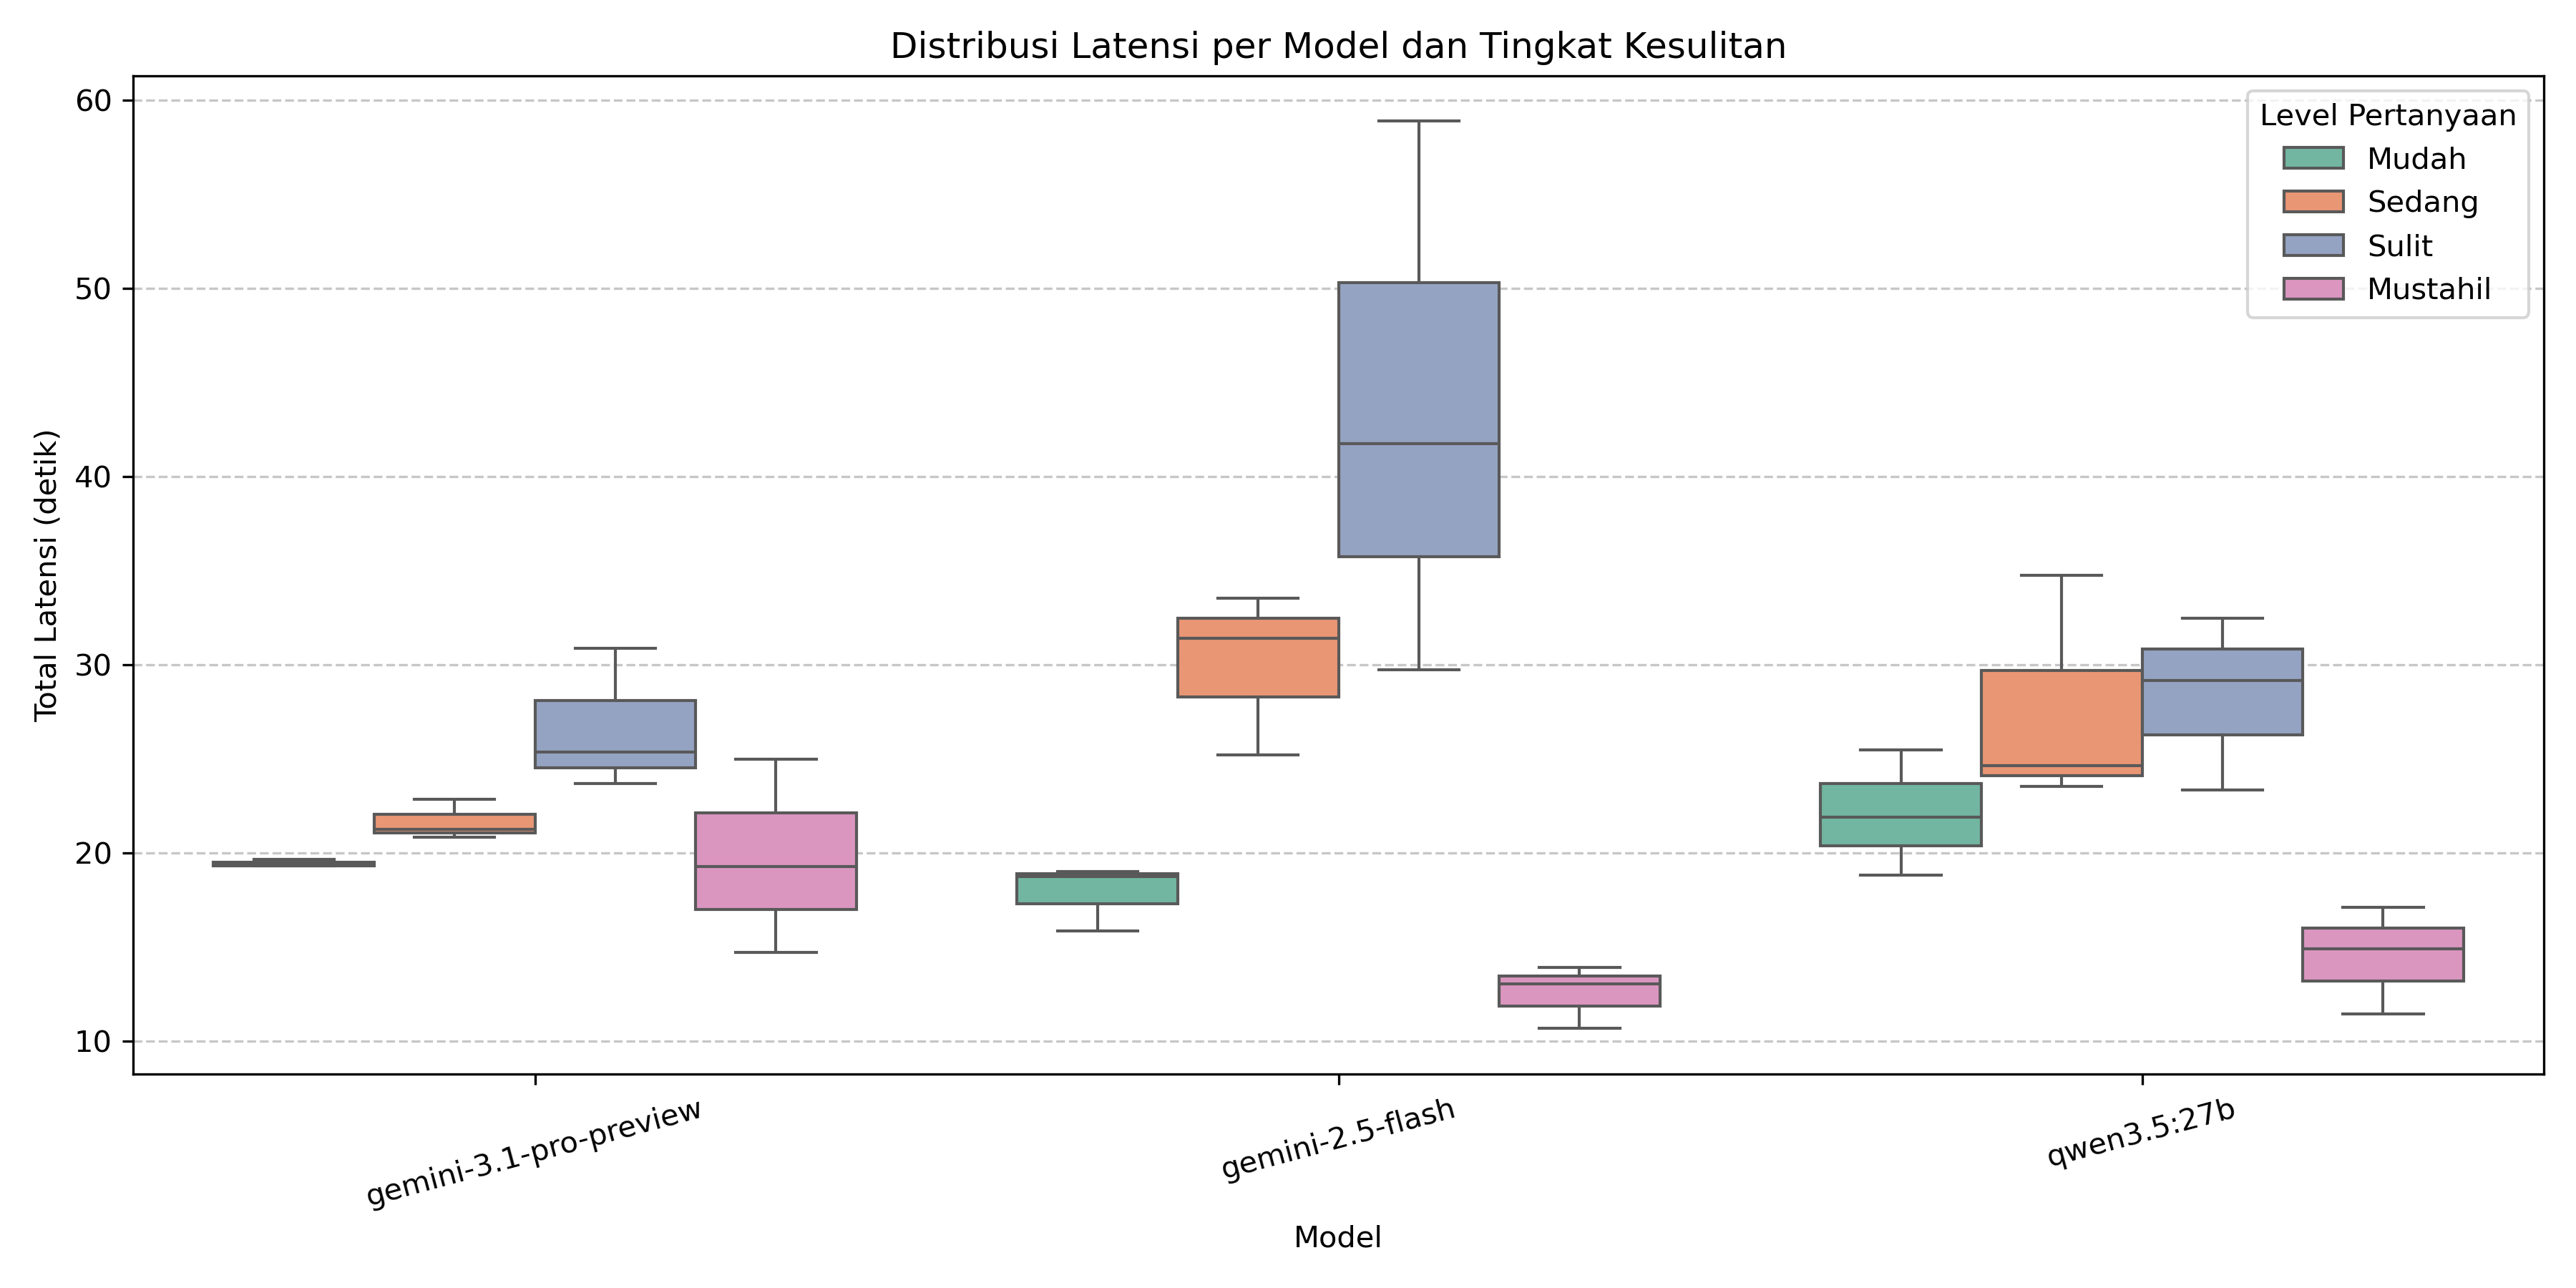
\includegraphics[width=0.8\textwidth]{Init/gambar/boxplots/boxplot_plan_latensi.png}
    \caption{Distribusi Latensi Pengujian Pembuatan \textit{Plan} per Model}
    \label{fig:boxplot_plan_latensi}
\footnotesize \textbf{Sumber:} Dokumentasi Penulis
\end{figure}

\begin{figure}[H]
    \centering
    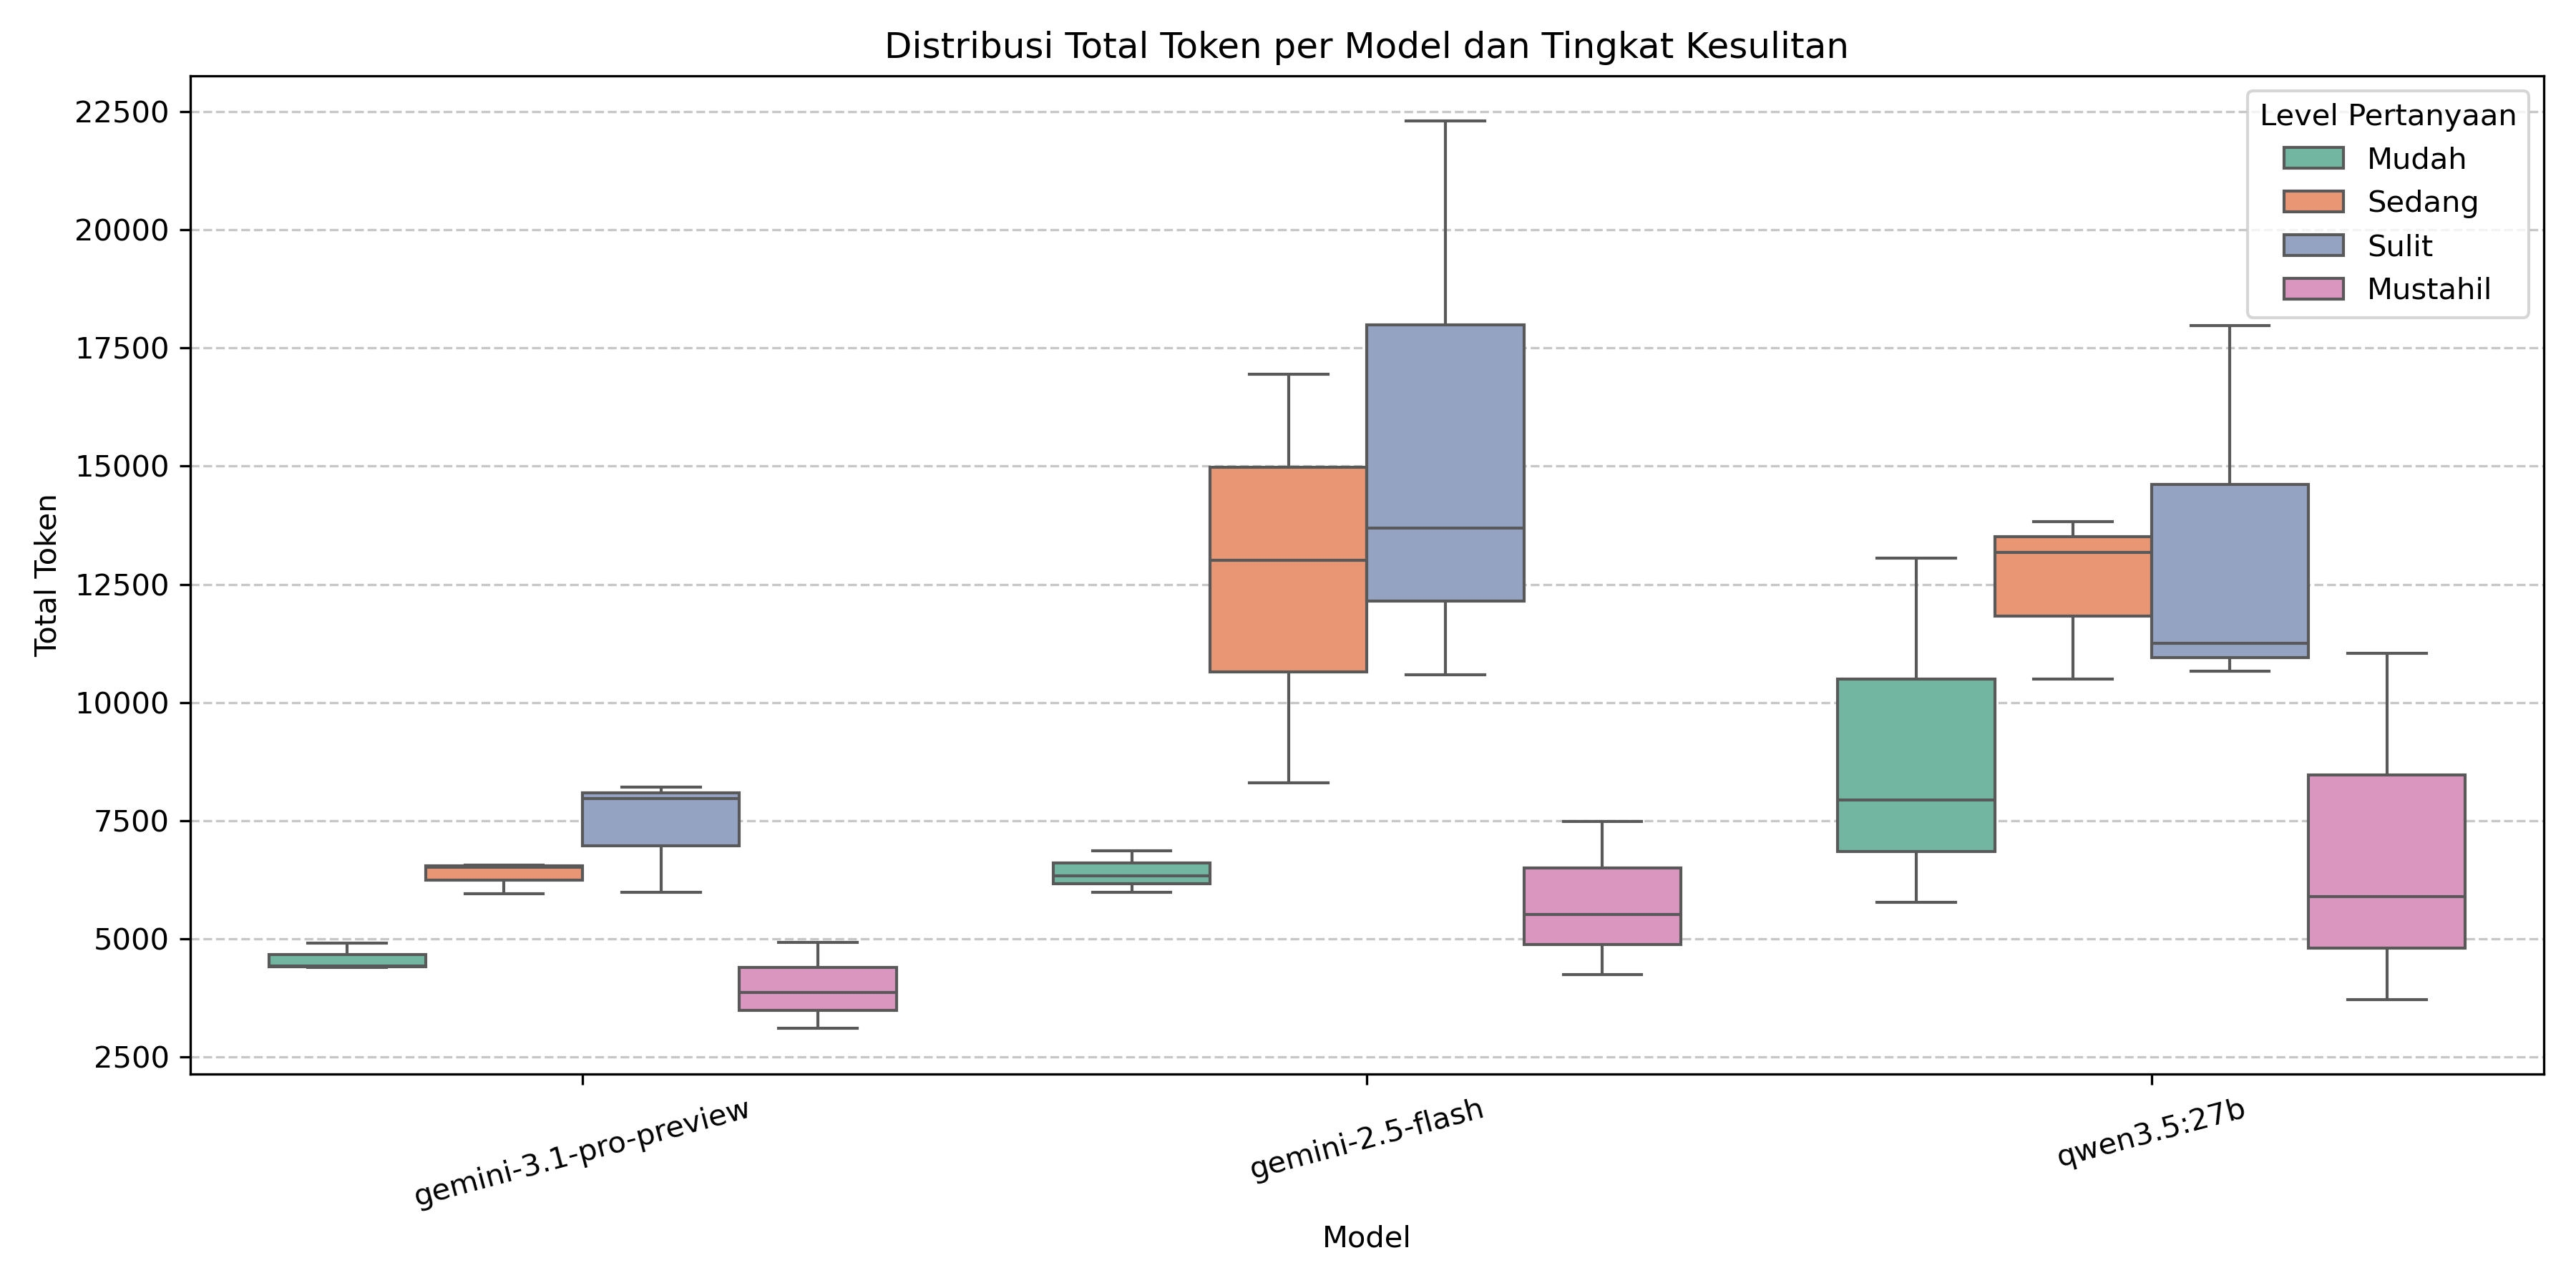
\includegraphics[width=0.8\textwidth]{Init/gambar/boxplots/boxplot_plan_token.png}
    \caption{Distribusi Konsumsi Token Pengujian Pembuatan \textit{Plan} per Model}
    \label{fig:boxplot_plan_token}
\footnotesize \textbf{Sumber:} Dokumentasi Penulis
\end{figure}


\subsection{Analisis Data Keberhasilan}
Berdasarkan hasil pengujian pada Tabel \ref{tab:plan_results}, kemampuan model dalam menyusun \textit{plan} inspeksi dievaluasi tidak hanya dari ketepatan pembuatan \textit{plan}, melainkan juga dari kemampuan penalaran matematis dan spasial untuk menyusun \textit{plan} yang efisien. Gemini 3.1 Pro Preview kembali menunjukkan dominasinya dengan tingkat keberhasilan skor dan rute terpendek mencapai 100\% di seluruh tingkat kesulitan. Sebaliknya, Gemini 2.5 Flash dan Qwen 3.5 mencatatkan tingkat keberhasilan pembuatan \textit{plan} sebesar 91,67\%, namun dengan tingkat efisiensi rute yang lebih rendah, yaitu 85,71\% untuk Flash dan 75,00\% untuk Qwen. Menariknya, ketiga model mencetak skor (100\%) pada level ``Mustahil'', menunjukkan kemampuan yang sangat baik dalam memvalidasi ketersediaan objek sebelum merencanakan rute, sehingga terhindar dari perencanaan halusinatif ketika objek yang diminta tidak ada di lingkungan.

Analisis terhadap kegagalan penyusunan rute pada Gemini 2.5 Flash dan Qwen 3.5 27B menunjukkan adanya satu kelemahan mendasar yang sama, yaitu kecenderungan menggunakan pendekatan \textit{greedy} yang berujung pada rute yang tidak optimal. Kedua model sering kali terjebak dengan hanya memilih objek terdekat dari posisi saat ini tanpa mempertimbangkan konsekuensi jarak akumulatif terhadap objek-objek selanjutnya. Pada Gemini 2.5 Flash, pendekatan ini menyebabkannya memilih objek terdekat yang justru menjauhkannya dari letak objek tujuan akhir, sehingga total jarak tempuh membengkak. Kesalahan identik juga dilakukan oleh Qwen 3.5, di mana model mengeksekusi inspeksi kumpulan objek searah secara berurutan, namun melewatkan satu objek di arah berlawanan, yang pada akhirnya memaksa robot melakukan manuver putar balik jarak jauh di akhir sesi. Kegagalan ini menegaskan bahwa kedua model tersebut memiliki keterbatasan arsitektur dalam memprediksi jarak secara menyeluruh.

Di sisi lain, Qwen 3.5 juga mengalami satu kegagalan berbeda terkait penalaran spasial, yang menyebabkan efisiensi rute menjadi lebih rendah dibandingkan model lainnya. Pada kasus tersebut, ketika dihadapkan pada beberapa kandidat objek, model tidak memilih objek terdekat untuk dimasukkan ke dalam rute, melainkan memilih objek yang posisinya lebih jauh dari kumpulan objek lainnya. Temuan ini menunjukkan bahwa pada kondisi tertentu Qwen 3.5 masih dapat mengalami kesalahan dalam membandingkan kedekatan spasial antar kandidat objek, yang berdampak pada kualitas rute inspeksi yang dihasilkan.

Selain permasalahan spasial tersebut, baik Gemini 2.5 Flash maupun Qwen 3.5 juga menunjukkan beberapa keterbatasan pada aspek lain. Gemini 2.5 Flash sempat gagal mematuhi batasan jumlah objek yang diinstruksikan, yaitu menyusun plan untuk tiga objek meskipun pengguna hanya meminta inspeksi terhadap satu objek. Sementara itu, Qwen 3.5 sempat mengalami kegagalan penyusunan plan akibat menghasilkan parameter yang tidak sesuai pada pemanggilan tool pencarian objek, sehingga tool tidak mengembalikan objek yang diharapkan.

\subsection{Analisis Latensi dan Konsumsi \textit{Token}}
Berdasarkan distribusi latensi (Gambar \ref{fig:boxplot_plan_latensi}) dan konsumsi token (Gambar \ref{fig:boxplot_plan_token}), terlihat pembalikan tren efisiensi dibandingkan kedua pengujian sebelumnya. Gemini 2.5 Flash, yang secara konsisten menjadi model tercepat dan paling efisien pada pengujian pemanggilan \textit{tool} murni maupun analisis \textit{image}, kini justru menunjukkan performa terburuk, latensi dan konsumsi tokennya melonjak, terutama pada level sedang dan sulit. Perubahan tren ini mengindikasikan bahwa Gemini 2.5 Flash membutuhkan proses penalaran yang lebih panjang ketika menangani perencanaan rute dengan banyak objek. Hal tersebut tercermin dari meningkatnya jumlah token yang dihasilkan, yang kemudian berdampak pada kenaikan latensi. Sebaliknya, Gemini 3.1 Pro justru menampilkan hasil yang paling efisien. Kemampuan penalaran pada Gemini Pro yang sebelumnya membuatnya tampak lebih lambat di pengujian dasar, kini terbukti lebih efisien untuk memecahkan masalah rute kompleks secara langsung tanpa memerlukan respon yang panjang. Sementara itu, Qwen 3.5 menunjukkan tren yang konsisten dengan pengujian sebelumnya, yakni mengonsumsi token dalam jumlah besar akibat format respons yang panjang, sehingga latensi inferensinya di server lokal pun tetap tinggi. Temuan ini menunjukkan bahwa efisiensi inferensi sangat dipengaruhi oleh kesesuaian antara karakteristik model dan kompleksitas tugas yang diberikan, model ringan yang dirancang untuk kecepatan, seperti Gemini Flash, akan mengalami pembengkakan token saat dipaksa menyelesaikan tugas penalaran tingkat tinggi, sementara model kompleks, seperti Gemini Pro, akan mengeksekusinya secara efisien.



% =============================================================================
% PENGUJIAN 4: KESELURUHAN SISTEM (END-TO-END)
% =============================================================================
\section{Pengujian Keseluruhan Sistem}
\label{sec:pengujian_e2e}

Pengujian ini bertujuan untuk mengevaluasi kinerja sistem secara menyeluruh dari awal hingga akhir (\textit{end-to-end}) dalam skenario inspeksi visual yang realistis. Pengujian mengukur kemampuan integrasi seluruh komponen sistem, mulai dari pembuatan rencana inspeksi, navigasi robot ke lokasi target, pengambilan dan analisis \textit{image}, hingga mekanisme intervensi operator (\textit{Human-in-the-Loop}).

\subsection{Skenario Pengujian}
Pengujian \textit{end-to-end} dirancang dalam tiga tingkat kesulitan (mudah, sedang, sulit) dengan tiga variasi skenario pada setiap tingkat. Lingkungan yang digunakan pada pengujian ini direpresentasikan oleh peta pada \textit{image} \ref{fig:map_annotated_e2e}. Pada peta tersebut, lokasi objek-objek inspeksi ditandai dengan lingkaran berwarna, di mana setiap jenis objek memiliki warna yang berbeda sesuai dengan keterangan pada legenda. Secara keseluruhan, terdapat 4 APAR, 3 stop kontak, dan 2 tong sampah yang tersebar di area pengujian. 

\begin{figure}[H]
    \centering
    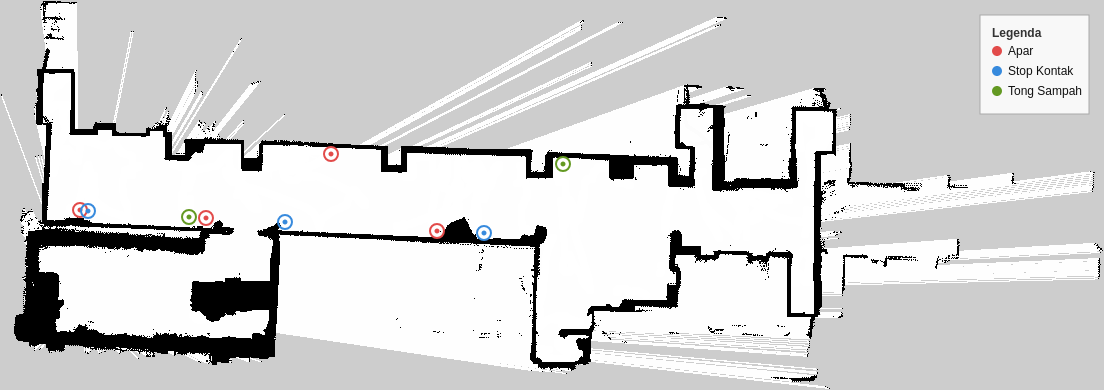
\includegraphics[width=0.8\textwidth]{Init/gambar/map_annotated.png}
    \caption{Peta Lingkungan Pengujian \textit{End-to-End} dengan Penanda Lokasi Objek}
    \label{fig:map_annotated_e2e}
\footnotesize \textbf{Sumber:} Dokumentasi Penulis
\end{figure}

Berikut adalah rincian seluruh skenario pengujian beserta instruksi awal yang diberikan kepada agen robot:

\renewcommand{\arraystretch}{1.5}
\begin{longtable}{|c|p{4cm}|p{8.5cm}|}
\caption{Detail Skenario Pengujian Keseluruhan Sistem (\textit{End-to-End})} \label{tab:skenario_e2e} \\
\hline
\textbf{Level} & \textbf{Skenario} & \textbf{Deskripsi dan Instruksi Pengguna} \\
\hline
\endfirsthead
\multicolumn{3}{c}%
{{Tabel \ref{tab:skenario_e2e} lanjutan dari halaman sebelumnya}} \\
\hline
\textbf{Level} & \textbf{Skenario} & \textbf{Deskripsi dan Instruksi Pengguna} \\
\hline
\endhead
\hline \multicolumn{3}{|r|}{{Lanjut ke halaman berikutnya}} \\ \hline
\endfoot
\hline
\endlastfoot

Mudah & Skenario 1 & Inspeksi 1 APAR berkondisi normal, Tanpa intervensi user. \newline \textbf{Instruksi:} \textit{``tolong inspeksi satu APAR terdekat di lantai 9''} \\
\cline{2-3}
& Skenario 2 & Inspeksi 1 APAR dengan anomali 'APAR di lantai', Tanpa intervensi user. \newline \textbf{Instruksi:} \textit{``tolong periksa kondisi satu APAR terdekat di lantai 9''} \\
\cline{2-3}
& Skenario 3 & Inspeksi 1 APAR dengan anomali 'selang tidak terpasang pada clip body', Dengan intervensi user mengubah plan sebelum dimulai (meminta robot duduk setelah inspeksi selesai). \newline \textbf{Instruksi:} \textit{``tolong inspeksi satu APAR terdekat di lantai 9''} \\
\hline

Sedang & Skenario 1 & Inspeksi 3 objek berbeda (1 APAR, 1 stop kontak, 1 tong sampah) yang semuanya normal, Tanpa intervensi user. \newline \textbf{Instruksi:} \textit{``tolong lakukan inspeksi pada satu APAR, satu stop kontak, dan satu tong sampah terdekat di lantai 9''} \\
\cline{2-3}
& Skenario 2 & Inspeksi 3 objek berbeda (1 APAR dengan anomali 'selang tidak terpasang pada clip body', 1 stop kontak dengan anomali 'terdapat steker', 1 tong sampah dengan anomali 'tong sampah berantakan banyak sampah'), Tanpa intervensi user. \newline \textbf{Instruksi:} \textit{``inspeksi satu APAR, satu stop kontak, dan satu tong sampah terdekat di lantai 9''} \\
\cline{2-3}
& Skenario 3 & Inspeksi objek berbeda (1 APAR dengan anomali 'selang tidak terpasang pada clip body', 1 stop kontak normal), Dengan intervensi user mengubah plan di tengah misi (saat robot di stop kontak, user minta penambahan inspeksi tong sampah). \newline \textbf{Instruksi:} \textit{``tolong periksa satu APAR, dan satu stop kontak terdekat di lantai 9''} \\
\hline

Sulit & Skenario 1 & Inspeksi 6 objek (2 APAR, 2 stop kontak, 2 tong sampah), Kondisi: 3 objek normal, 3 objek anomali (1 APAR di lantai, 1 steker rusak, 1 tong sampah tidak lengkap), Tanpa intervensi user. \newline \textbf{Instruksi:} \textit{``tolong lakukan inspeksi ke dua APAR, dua stop kontak, dan dua tong sampah terdekat di lantai 9''} \\
\cline{2-3}
& Skenario 2 & Inspeksi 6 objek (1 APAR normal, 1 APAR di lantai, 1 APAR dengan selang tidak terpasang pada clip body, 1 stop kontak dengan steker rusak, 1 tong sampah tidak lengkap, 1 tong sampah normal), Dengan intervensi user membatalkan 1 stop kontak dan menambah 1 tong sampah. \newline \textbf{Instruksi:} \textit{``tolong inspeksi tiga APAR, dua stop kontak, dan satu tong sampah terdekat di lantai 9''} \\
\cline{2-3}
& Skenario 3 & Inspeksi 6 objek (1 APAR normal, 1 APAR di lantai, 2 APAR dengan selang tidak terpasang pada clip body, 1 stop kontak normal, 1 tong sampah dengan sampah berserakan), Dengan intervensi user, saat robot sampai di salah satu APAR yang memiliki anomali, user menginstruksikan robot untuk maju mendekat. \newline \textbf{Instruksi:} \textit{``tolong periksa empat APAR, satu stop kontak, dan satu tong sampah terdekat di lantai 9''} \\
\end{longtable}

Parameter evaluasi meliputi keberhasilan pembuatan \textit{plan}, keberhasilan \textit{plan} jarak terpendek, keberhasilan analisis objek, keberhasilan penanganan intervensi, total waktu sesi, total token sesi, dan jumlah pemanggilan \textit{tool}.

\subsection{Hasil Pengujian}

% --- Tabel Ringkasan E2E ---
\begin{table}[H]
\centering
\caption{Ringkasan Hasil Pengujian \textit{End-to-End}}
\label{tab:e2e_summary}
\renewcommand{\arraystretch}{1.2}
\resizebox{\linewidth}{!}{
\begin{tabular}{|l|c|c|c|}
\hline
\textbf{Metrik} & \textbf{Gemini 2.5 Flash} & \textbf{Gemini 3.1 Pro} & \textbf{Qwen 3.5 27B} \\
\hline
Keberhasilan \textit{Plan} & 100,00\% & 100,00\% & 100,00\% \\
\hline
\textit{Plan} Rute Terpendek & 77,78\% & 100,00\% & 66,67\% \\
\hline
Keberhasilan Analisis Objek & 86,67\% & 93,33\% & 63,33\% \\
\hline
Keberhasilan Intervensi & 100,00\% & 100,00\% & 100,00\% \\
\hline
Rata-rata Waktu Sesi (detik) & 382,91 & 367,40 & 610,79 \\
\hline
Rata-rata Konsumsi Token & 153.564 & 183.440 & 140.072 \\
\hline
\end{tabular}
}
\end{table}

% --- Tabel Hasil E2E Gemini 2.5 Flash ---
\begin{longtable}{|c|c|c|c|c|c|c|c|}
\caption{Hasil Pengujian \textit{End-to-End} Model Gemini 2.5 Flash} \label{tab:e2e_flash} \\
\hline
\textbf{Level} & \textbf{Skenario} & \textbf{Plan} & \textbf{Rute} & \textbf{Analisis} & \textbf{Intervensi} & \textbf{Waktu (s)} & \textbf{Token} \\
\hline
\endfirsthead
\hline
\textbf{Level} & \textbf{Skenario} & \textbf{Plan} & \textbf{Rute} & \textbf{Analisis} & \textbf{Intervensi} & \textbf{Waktu (s)} & \textbf{Token} \\
\hline
\endhead
Mudah & 1 & \checkmark & \checkmark & 1/1 & -- & 84,89 & 34.922 \\
\hline
Mudah & 2 & \checkmark & \checkmark & 1/1 & -- & 64,54 & 32.876 \\
\hline
Mudah & 3 & \checkmark & \checkmark & 1/1 & \checkmark & 150,29 & 52.467 \\
\hline
Sedang & 1 & \checkmark & \checkmark & 3/3 & -- & 295,61 & 125.978 \\
\hline
Sedang & 2 & \checkmark & \checkmark & 2/3 & -- & 285,75 & 111.419 \\
\hline
Sedang & 3 & \checkmark & \checkmark & 3/3 & \checkmark & 335,43 & 126.673 \\
\hline
Sulit & 1 & \checkmark & \checkmark & 6/6 & -- & 591,96 & 248.842 \\
\hline
Sulit & 2 & \checkmark & $\times$ & 5/6 & \checkmark & 775,59 & 279.289 \\
\hline
Sulit & 3 & \checkmark & $\times$ & 4/6 & \checkmark & 862,10 & 369.609 \\
\hline
\end{longtable}

% --- Tabel Hasil E2E Gemini 3.1 Pro ---
\begin{longtable}{|c|c|c|c|c|c|c|c|}
\caption{Hasil Pengujian \textit{End-to-End} Model Gemini 3.1 Pro Preview} \label{tab:e2e_pro} \\
\hline
\textbf{Level} & \textbf{Skenario} & \textbf{Plan} & \textbf{Rute} & \textbf{Analisis} & \textbf{Intervensi} & \textbf{Waktu (s)} & \textbf{Token} \\
\hline
\endfirsthead
\hline
\textbf{Level} & \textbf{Skenario} & \textbf{Plan} & \textbf{Rute} & \textbf{Analisis} & \textbf{Intervensi} & \textbf{Waktu (s)} & \textbf{Token} \\
\hline
\endhead
Mudah & 1 & \checkmark & \checkmark & 1/1 & -- & 110,43 & 30.631 \\
\hline
Mudah & 2 & \checkmark & \checkmark & 1/1 & -- & 93,48 & 30.898 \\
\hline
Mudah & 3 & \checkmark & \checkmark & 1/1 & \checkmark & 145,12 & 45.712 \\
\hline
Sedang & 1 & \checkmark & \checkmark & 3/3 & -- & 294,14 & 173.103 \\
\hline
Sedang & 2 & \checkmark & \checkmark & 3/3 & -- & 277,23 & 115.623 \\
\hline
Sedang & 3 & \checkmark & \checkmark & 3/3 & \checkmark & 250,91 & 128.318 \\
\hline
Sulit & 1 & \checkmark & \checkmark & 6/6 & -- & 681,65 & 318.511 \\
\hline
Sulit & 2 & \checkmark & \checkmark & 5/6 & \checkmark & 560,26 & 332.709 \\
\hline
Sulit & 3 & \checkmark & \checkmark & 5/6 & \checkmark & 893,42 & 475.459 \\
\hline
\end{longtable}

% --- Tabel Hasil E2E Qwen 3.5 ---
\begin{longtable}{|c|c|c|c|c|c|c|c|}
\caption{Hasil Pengujian \textit{End-to-End} Model Qwen 3.5 27B} \label{tab:e2e_qwen} \\
\hline
\textbf{Level} & \textbf{Skenario} & \textbf{Plan} & \textbf{Rute} & \textbf{Analisis} & \textbf{Intervensi} & \textbf{Waktu (s)} & \textbf{Token} \\
\hline
\endfirsthead
\hline
\textbf{Level} & \textbf{Skenario} & \textbf{Plan} & \textbf{Rute} & \textbf{Analisis} & \textbf{Intervensi} & \textbf{Waktu (s)} & \textbf{Token} \\
\hline
\endhead
Mudah & 1 & \checkmark & \checkmark & 1/1 & -- & 105,29 & 25.678 \\
\hline
Mudah & 2 & \checkmark & \checkmark & 0/1 & -- & 100,85 & 31.529 \\
\hline
Mudah & 3 & \checkmark & \checkmark & 0/1 & \checkmark & 186,36 & 60.081 \\
\hline
Sedang & 1 & \checkmark & \checkmark & 3/3 & -- & 374,77 & 99.721 \\
\hline
Sedang & 2 & \checkmark & \checkmark & 2/3 & -- & 274,29 & 102.818 \\
\hline
Sedang & 3 & \checkmark & \checkmark & 3/3 & \checkmark & 397,54 & 108.792 \\
\hline
Sulit & 1 & \checkmark & $\times$ & 4/6 & -- & 1.550,64 & 231.210 \\
\hline
Sulit & 2 & \checkmark & $\times$ & 3/6 & \checkmark & 1.010,24 & 224.071 \\
\hline
Sulit & 3 & \checkmark & $\times$ & 3/6 & \checkmark & 1.497,17 & 376.747 \\
\hline
\end{longtable}
\begin{figure}[H]
    \centering
    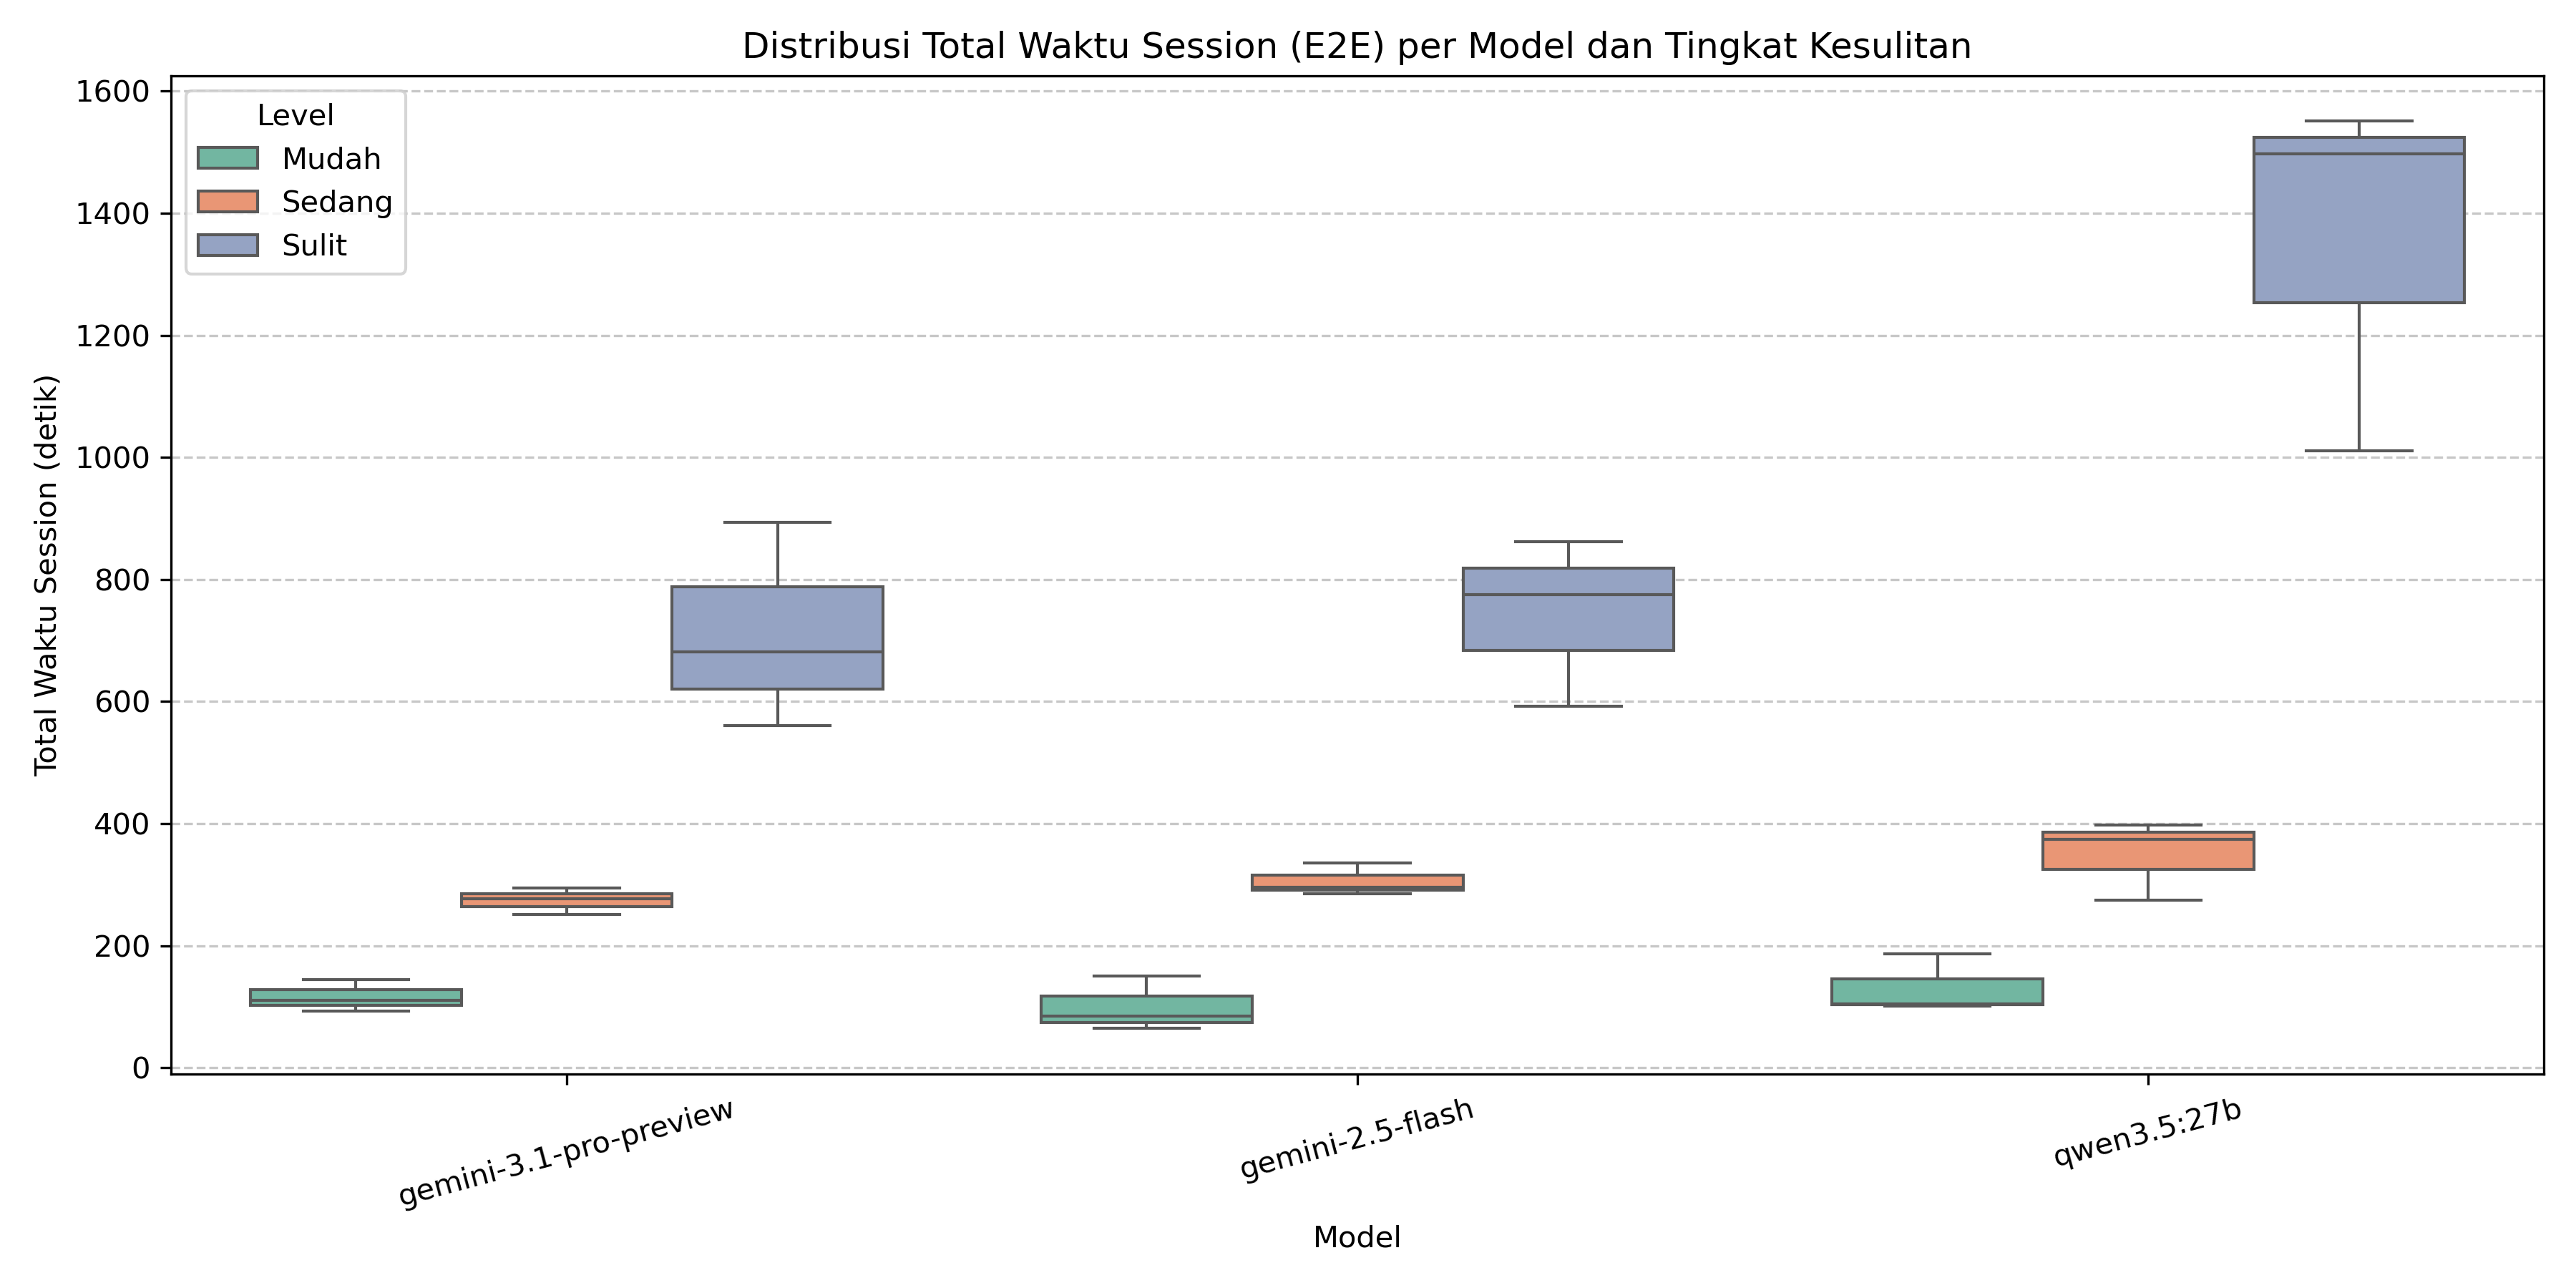
\includegraphics[width=0.8\textwidth]{Init/gambar/boxplots/boxplot_e2e_latensi.png}
    \caption{Distribusi Waktu Sesi Pengujian \textit{End-to-End} per Model}
    \label{fig:boxplot_e2e_latensi}
\footnotesize \textbf{Sumber:} Dokumentasi Penulis
\end{figure}

\begin{figure}[H]
    \centering
    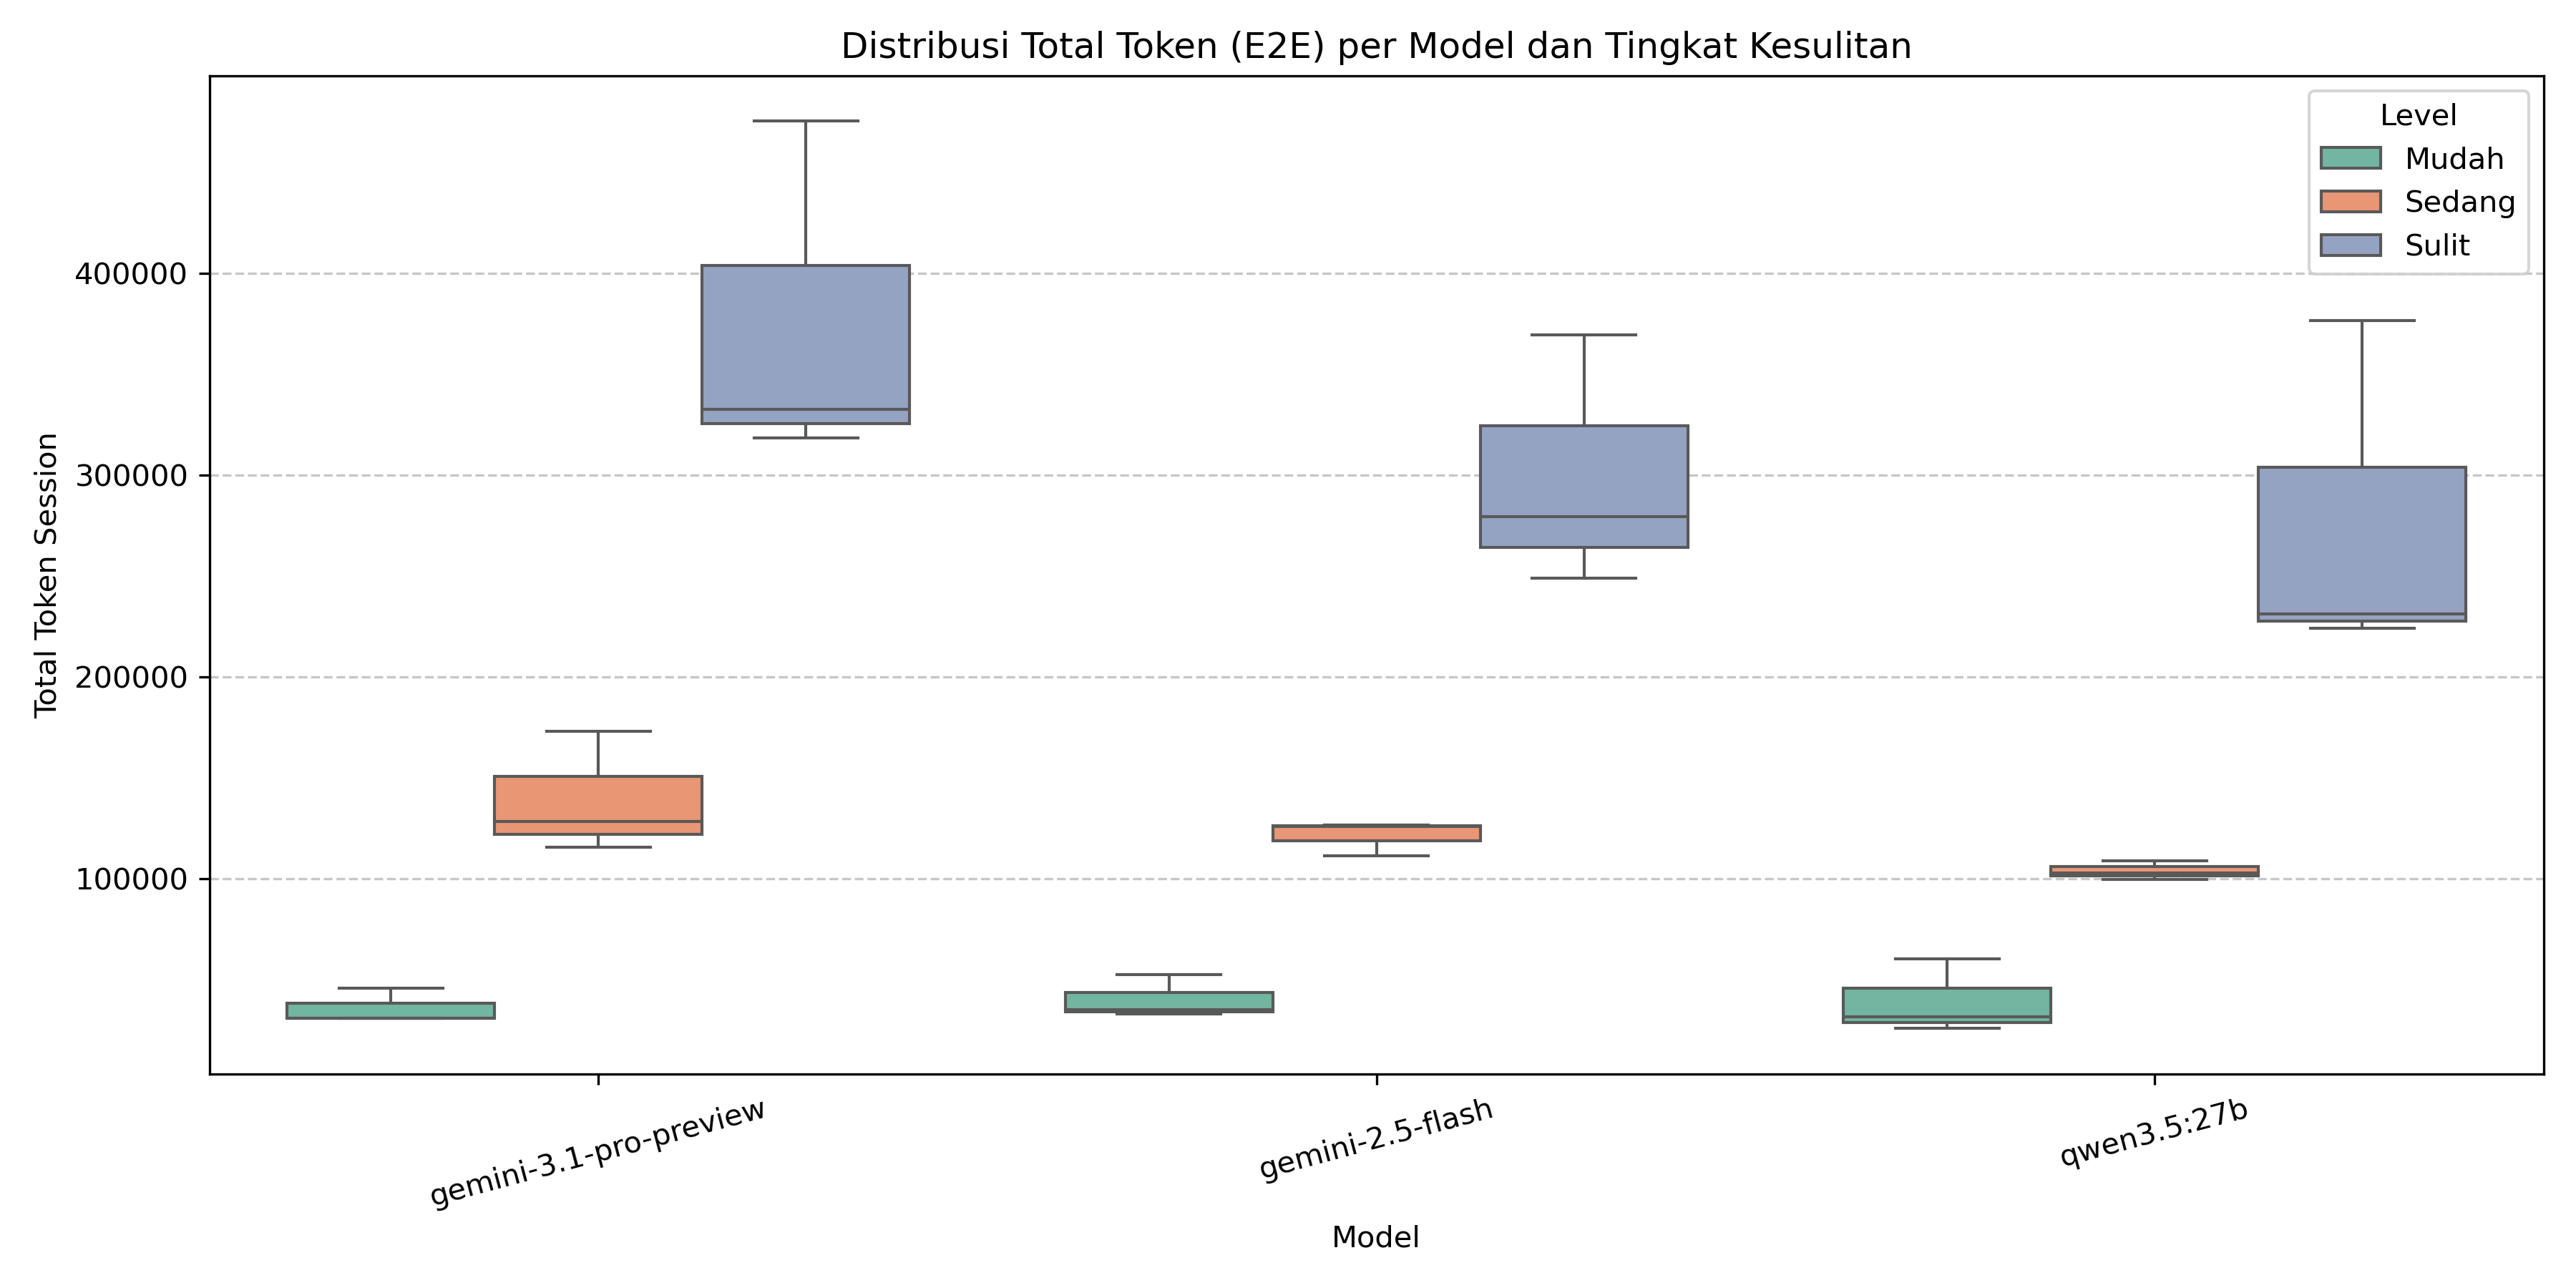
\includegraphics[width=0.8\textwidth]{Init/gambar/boxplots/boxplot_e2e_token.png}
    \caption{Distribusi Konsumsi Token Pengujian \textit{End-to-End} per Model}
    \label{fig:boxplot_e2e_token}
\footnotesize \textbf{Sumber:} Dokumentasi Penulis
\end{figure}

\subsection{Analisis Data Keberhasilan}
Berdasarkan hasil pengujian pada Tabel \ref{tab:e2e_summary}, \ref{tab:e2e_flash}, \ref{tab:e2e_pro}, dan \ref{tab:e2e_qwen}, sistem inspeksi otonom menunjukkan tingkat keberhasilan dasar yang tinggi. Ketiga model berhasil mencatatkan persentase 100\% pada keberhasilan pembuatan \textit{plan} awal di seluruh variasi skenario, termasuk saat terjadi intervensi operator. Hal ini membuktikan bahwa integrasi agen MLLM berjalan stabil dalam mengonversi keputusan teks menjadi aksi pergerakan fisik robot. Seluruh model juga terbukti adaptif dalam merespons instruksi intervensi operator, baik berupa perubahan rencana, instruksi manuver tambahan, maupun penambahan objek baru di tengah misi. Sedangkan, dalam aspek perencanaan rute, Gemini 3.1 Pro terbukti sangat andal dengan mempertahankan rekor 100\% rute terpendek. Di sisi lain, keterbatasan arsitektur penalaran spasial pada Gemini 2.5 Flash dan Qwen 3.5 kembali terlihat jelas. Flash gagal menentukan rute paling efisien pada skenario Sulit Skenario 2 dan Skenario 3 akibat pola pendekatan \textit{greedy} yang tidak optimal, sementara Qwen 3.5 secara konsisten gagal menyusun rute terpendek di seluruh skenario level Sulit.

Perbedaan performa antar model terlihat signifikan pada evaluasi akurasi analisis visual di lapangan. Gemini 3.1 Pro Preview kembali menjadi yang terbaik dengan keberhasilan analisis objek mencapai 93,33\% dari keseluruhan objek uji di berbagai skenario. Dua kegagalan analisis pada model ini hanya terjadi pada skenario Sulit Skenario 2 (salah mengidentifikasi APAR merah menjadi kuning) dan Sulit Skenario 3 (salah mengidentifikasi selang APAR normal menjadi terlepas). Di urutan kedua, Gemini 2.5 Flash mencatatkan keberhasilan sebesar 86,67\%. Analisis menunjukkan pola kegagalan yang konsisten, khususnya pada deteksi warna APAR. Pada skenario Sedang Skenario 2 Gemini 2.5 Flash dan Sulit Skenario 2 Gemini 3.1 Pro, MLLM menyimpulkan bahwa tabung APAR berwarna kuning. Menariknya, kesalahan deteksi akibat dominasi piksel kuning dari stiker label ini sebelumnya hanya dialami oleh model Qwen 3.5 pada pengujian analisis \textit{image}. Fakta bahwa kedua varian Gemini akhirnya ikut terdistraksi oleh jebakan visual yang sama menegaskan bahwa kerentanan terhadap dominasi warna mayoritas merupakan kelemahan bawaan  pada MLLM. Meskipun SOP telah dirancang secara eksplisit untuk mengabaikan warna label, MLLM secara general ada kalanya tetap terkecoh dan mengabaikan instruksi pengecualian tersebut. Selain masalah warna, Flash juga keliru menyatakan selang APAR menempel rapi pada klipnya pada skenario Sulit Skenario 3.

Sementara itu, Qwen 3.5 27B mengalami degradasi performa analisis visual yang sangat drastis dalam skenario \textit{end-to-end}, dengan tingkat keberhasilan hanya mencapai 63,33\%. Qwen berulang kali menghasilkan \textit{false positive}. Pada tingkat Mudah, model ini gagal mendeteksi anomali APAR yang jatuh di lantai dan menganggapnya tergantung normal di dinding, serta menganggap selang yang terlepas sebagai kondisi normal. Kegagalan ini terus berulang di level Sedang dan Sulit. Selain kelemahan pemahaman spasial, Qwen 3.5 juga mengalami kesalahan persepsi warna, menyatakan warna APAR pudar padahal aman. Secara umum, tingginya penurunan persentase keberhasilan analisis objek pada pengujian \textit{end-to-end} secara kuantitatif, terutama pada Qwen 3.5 dan Gemini 2.5 Flash, sebenarnya sangat dipengaruhi oleh komposisi \textit{dataset} skenario. Pengujian \textit{end-to-end} melibatkan repetisi yang jauh lebih tinggi untuk skenario anomali "selang APAR tidak menempel pada klip \textit{body}". Pada pengujian analisis \textit{image} sebelumnya, anomali struktural ini telah terbukti sebagai kasus spasial yang paling menantang dan paling sering mengecoh pemahaman spasial MLLM. Dengan tingginya frekuensi kemunculan skenario tersebut di sepanjang pengujian \textit{end-to-end}, performa kuantitatif model secara matematis akan mengalami penurunan yang signifikan.

\subsection{Analisis Waktu Sesi dan Konsumsi \textit{Token}}
Berdasarkan distribusi waktu sesi (Gambar \ref{fig:boxplot_e2e_latensi}) dan konsumsi token (Gambar \ref{fig:boxplot_e2e_token}), ditemukan sebuah anomali performa latensi yang membedakan pengujian keseluruhan sistem dengan pengujian terisolasi. Dari sisi waktu penyelesaian misi, Gemini 2.5 Flash awalnya berhasil menunjukkan latensi tercepat tingkat Mudah. Namun, pada level Sedang dan Sulit, latensi Flash meningkat drastis hingga menyamai bahkan melampaui lambatnya waktu eksekusi Gemini 3.1 Pro. Temuan ini sangat kontraintuitif dengan hasil pengujian analisis \textit{image} terisolasi sebelumnya, di mana Flash terbukti jauh lebih cepat memproses input visual dibandingkan Pro. Mengingat pada skenario \textit{end-to-end} proses pembuatan \textit{plan} hanya dieksekusi satu kali di awal misi, sedangkan pemanggilan \textit{tool} analisis \textit{image} dieksekusi berulang kali di setiap titik, secara matematis Flash seharusnya mendominasi kecepatan misi secara keseluruhan. Berkurangnya keunggulan waktu Flash secara signifikan ini kemungkinan disebabkan oleh adanya latensi jaringan yang tidak sama antara Gemini Flash dan Pro saat pengujian berlangsung. Hal inilah yang menyebabkan waktu eksekusi keseluruhan Flash seolah-olah tersusul dan melambat jika dibandingkan dengan Pro.

Di sisi lain, Qwen 3.5 mencatatkan waktu sesi yang sangat tinggi pada level Sulit, berkisar antara 17 hingga 26 menit. Lamanya waktu eksekusi ini merupakan akumulasi dari dua faktor utama, yaitu kelemahan inferensi Qwen pada pengujian analisis \textit{image}, di mana latensi ekstraksi fitur visual beruntun untuk banyak objek memberikan beban komputasi. Dari sisi konsumsi token, terlihat perbedaan tren yang menarik. Jika pada pengujian terisolasi Qwen 3.5 atau Gemini Flash sering menjadi yang paling boros token, pada skenario \textit{end-to-end} Gemini 3.1 Pro justru mencatatkan konsumsi token yang lebih tinggi. Penelusuran pada kode \textit{backend} mengonfirmasi bahwa perbedaan ini tidak semata-mata disebabkan oleh performa model, melainkan oleh berbedanya mekanisme serialisasi \textit{tool response} pada protokol API. Meskipun \textit{payload} balasan yang dikirimkan ke model adalah identik, Gemini API membungkus hasil \textit{tool} secara terstruktur menggunakan Part.from\_function\_response, sementara \textit{endpoint} Qwen 3.5 cukup menyerialisasinya menjadi string JSON standar melalui json.dumps(). Perbedaan format ini membuat Gemini secara tak terduga menghabiskan jauh lebih banyak token saat memproses hasil \textit{tool} dengan struktur data bersarang, sehingga selisih konsumsi token akhir pada pengujian \textit{end-to-end} ini sebagian besar merupakan konsekuensi dari penumpukan konteks respon \textit{tool}.



% =============================================================================
% PENGUJIAN 5: NASA-TLX
% =============================================================================
\section{Pengujian Beban Kerja Operator (NASA-TLX)}
\label{sec:pengujian_nasa_tlx}

Pengujian ini bertujuan untuk mengukur beban kerja yang dirasakan oleh operator saat menjalankan misi inspeksi menggunakan metode NASA Task Load Index (NASA-TLX). Hasil pengujian ini digunakan untuk mengevaluasi sejauh mana sistem yang dikembangkan dapat mengurangi beban kerja operator dibandingkan dengan metode inspeksi konvensional.

\subsection{Skenario Pengujian}
Pengujian dilakukan dengan melibatkan 10 responden yang masing-masing diminta untuk mengevaluasi beban kerja pada tiga kondisi inspeksi yang berbeda:

\begin{enumerate}
    \item \textbf{Inspeksi Keseluruhan Manual}: Operator mengendalikan robot secara penuh menggunakan teleoperasi manual untuk navigasi, pengambilan \textit{image}, dan analisis visual secara mandiri tanpa bantuan sistem AI.
    \item \textbf{Navigasi Otomatis + Analisis Visual Manual}: Operator menggunakan sistem \textit{chatbot} untuk menginstruksikan robot menghampiri objek secara otomatis, namun proses analisis visual kondisi objek masih dilakukan secara manual oleh operator.
    \item \textbf{Inspeksi Keseluruhan Otomatis}: Operator menggunakan sistem secara penuh, di mana baik navigasi maupun analisis visual objek dilakukan secara otomatis oleh sistem AI, dan operator hanya berperan sebagai pengawas.
\end{enumerate}

Ketiga kondisi pengujian di atas menggunakan skenario inspeksi yang sama, yaitu melakukan inspeksi terhadap tiga objek yang terdiri dari, satu APAR yang tergeletak di lantai, satu stop kontak dengan steker kabel terputus, dan satu tong sampah yang tidak lengkap. Pada kondisi pertama dan kedua, di mana analisis visual masih dilakukan secara manual, responden diminta untuk mengisi hasil analisis kondisi objek ke dalam lembar kerja Excel untuk merepresentasikan proses pelaporan inspeksi aslinya. Sedangkan pada kondisi ketiga, responden tidak perlu mengisi laporan tersebut karena analisis kondisi objek telah ditangani sepenuhnya oleh \textit{Multimodal Large Language Model}.

Setiap responden mengisi kuesioner NASA-TLX yang terdiri dari enam dimensi beban kerja, yaitu Kebutuhan Mental (\textit{Mental Demand}), Kebutuhan Fisik (\textit{Physical Demand}), Kebutuhan Waktu (\textit{Temporal Demand}), Performansi (\textit{Performance}), Usaha (\textit{Effort}), dan Tingkat Frustrasi (\textit{Frustration Level}). Setiap dimensi dinilai pada skala 0--100. Bobot kepentingan relatif antar dimensi ditentukan melalui prosedur perbandingan berpasangan (\textit{pairwise comparison}), menghasilkan bobot 0--5 untuk setiap dimensi. Skor akhir NASA-TLX dihitung menggunakan rumus \textit{Weighted Workload} (WWL):

\begin{equation}
\text{Skor NASA-TLX} = \frac{\sum_{i=1}^{6} (Bobot_i \times Rating_i)}{15}
\label{eq:nasa_tlx}
\end{equation}

\subsection{Profil Responden}

Gambar \ref{fig:dokumentasi_responden} menampilkan dokumentasi salah satu responden saat menjalankan skenario pengujian inspeksi.

\begin{figure}[H]
    \centering
    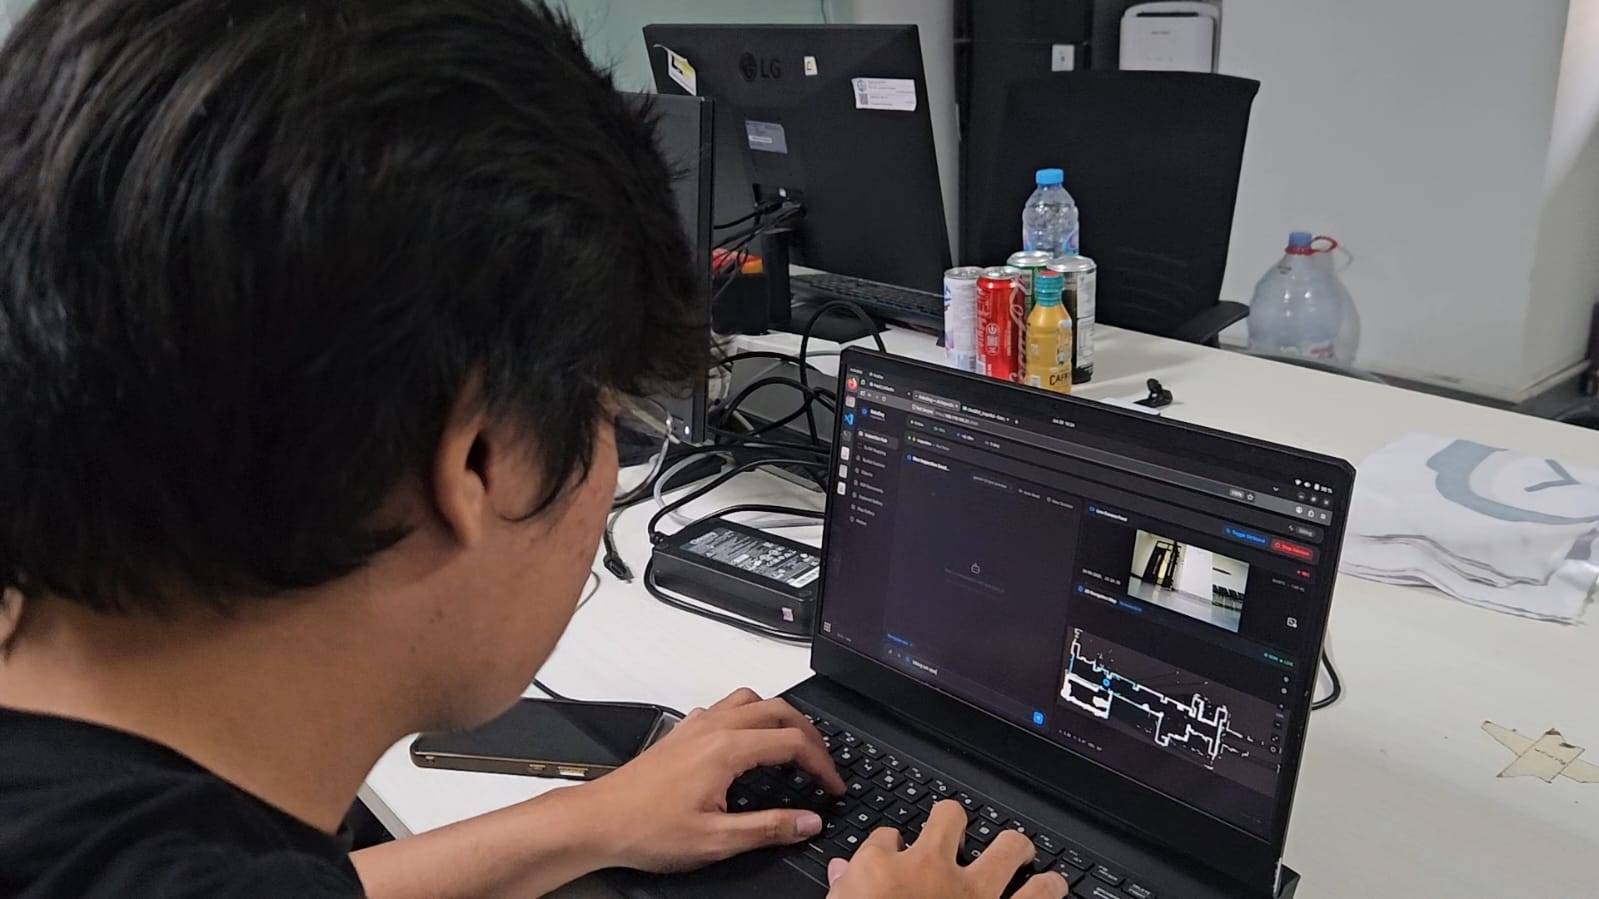
\includegraphics[width=0.8\textwidth]{Init/gambar/responden.jpeg}
    \caption{Dokumentasi Pelaksanaan Pengujian NASA-TLX oleh Responden}
    \label{fig:dokumentasi_responden}
\footnotesize \textbf{Sumber:} Dokumentasi Penulis
\end{figure}

\begin{table}[H]
\centering
\caption{Profil Demografi Responden NASA-TLX}
\label{tab:profil_responden}
\begin{tabular}{|c|l|c|c|l|l|}
\hline
\textbf{No} & \textbf{Nama} & \textbf{Usia} & \textbf{Gender} & \textbf{Pengalaman Robot} & \textbf{Familiaritas AI} \\
\hline
1 & Responden 1 & 21 & L & Pemula & Sangat Familiar \\
\hline
2 & Responden 2 & 22 & P & Pemula & Sangat Familiar \\
\hline
3 & Responden 3 & 22 & L & Pemula & Cukup Familiar \\
\hline
4 & Responden 4 & 22 & L & Tidak Pernah & Cukup Familiar \\
\hline
5 & Responden 5 & 21 & L & Tidak Pernah & Sangat Familiar \\
\hline
6 & Responden 6 & 19 & P & Pemula & Sangat Familiar \\
\hline
7 & Responden 7 & 19 & P & Pemula & Cukup Familiar \\
\hline
8 & Responden 8 & 20 & L & Pemula & Sangat Familiar \\
\hline
9 & Responden 9 & 22 & L & Tidak Pernah & Sangat Familiar \\
\hline
10 & Responden 10 & 22 & L & Tidak Pernah & Sangat Familiar \\
\hline
\end{tabular}
\end{table}

\subsection{Hasil Pengujian}

\begin{table}[H]
\centering
\caption{Skor NASA-TLX per Responden untuk Setiap Kondisi Inspeksi}
\label{tab:nasa_tlx_scores}
\begin{tabular}{|c|c|c|c|}
\hline
\textbf{Responden} & \textbf{Manual} & \textbf{Nav. Otomatis} & \textbf{Full Otomatis} \\
\hline
1 & 72,67 & 50,00 & 38,67 \\
\hline
2 & 45,33 & 43,00 & 19,67 \\
\hline
3 & 45,33 & 12,33 & 5,00 \\
\hline
4 & 23,33 & 41,67 & 2,67 \\
\hline
5 & 43,33 & 26,00 & 12,67 \\
\hline
6 & 75,67 & 42,33 & 35,33 \\
\hline
7 & 48,33 & 54,67 & 11,33 \\
\hline
8 & 80,00 & 26,67 & 23,00 \\
\hline
9 & 91,33 & 43,67 & 13,33 \\
\hline
10 & 16,00 & 5,33 & 22,33 \\
\hline
\hline
\textbf{Rata-rata} & \textbf{54,13} & \textbf{34,57} & \textbf{18,40} \\
\hline
\end{tabular}
\end{table}

\begin{figure}[H]
    \centering
    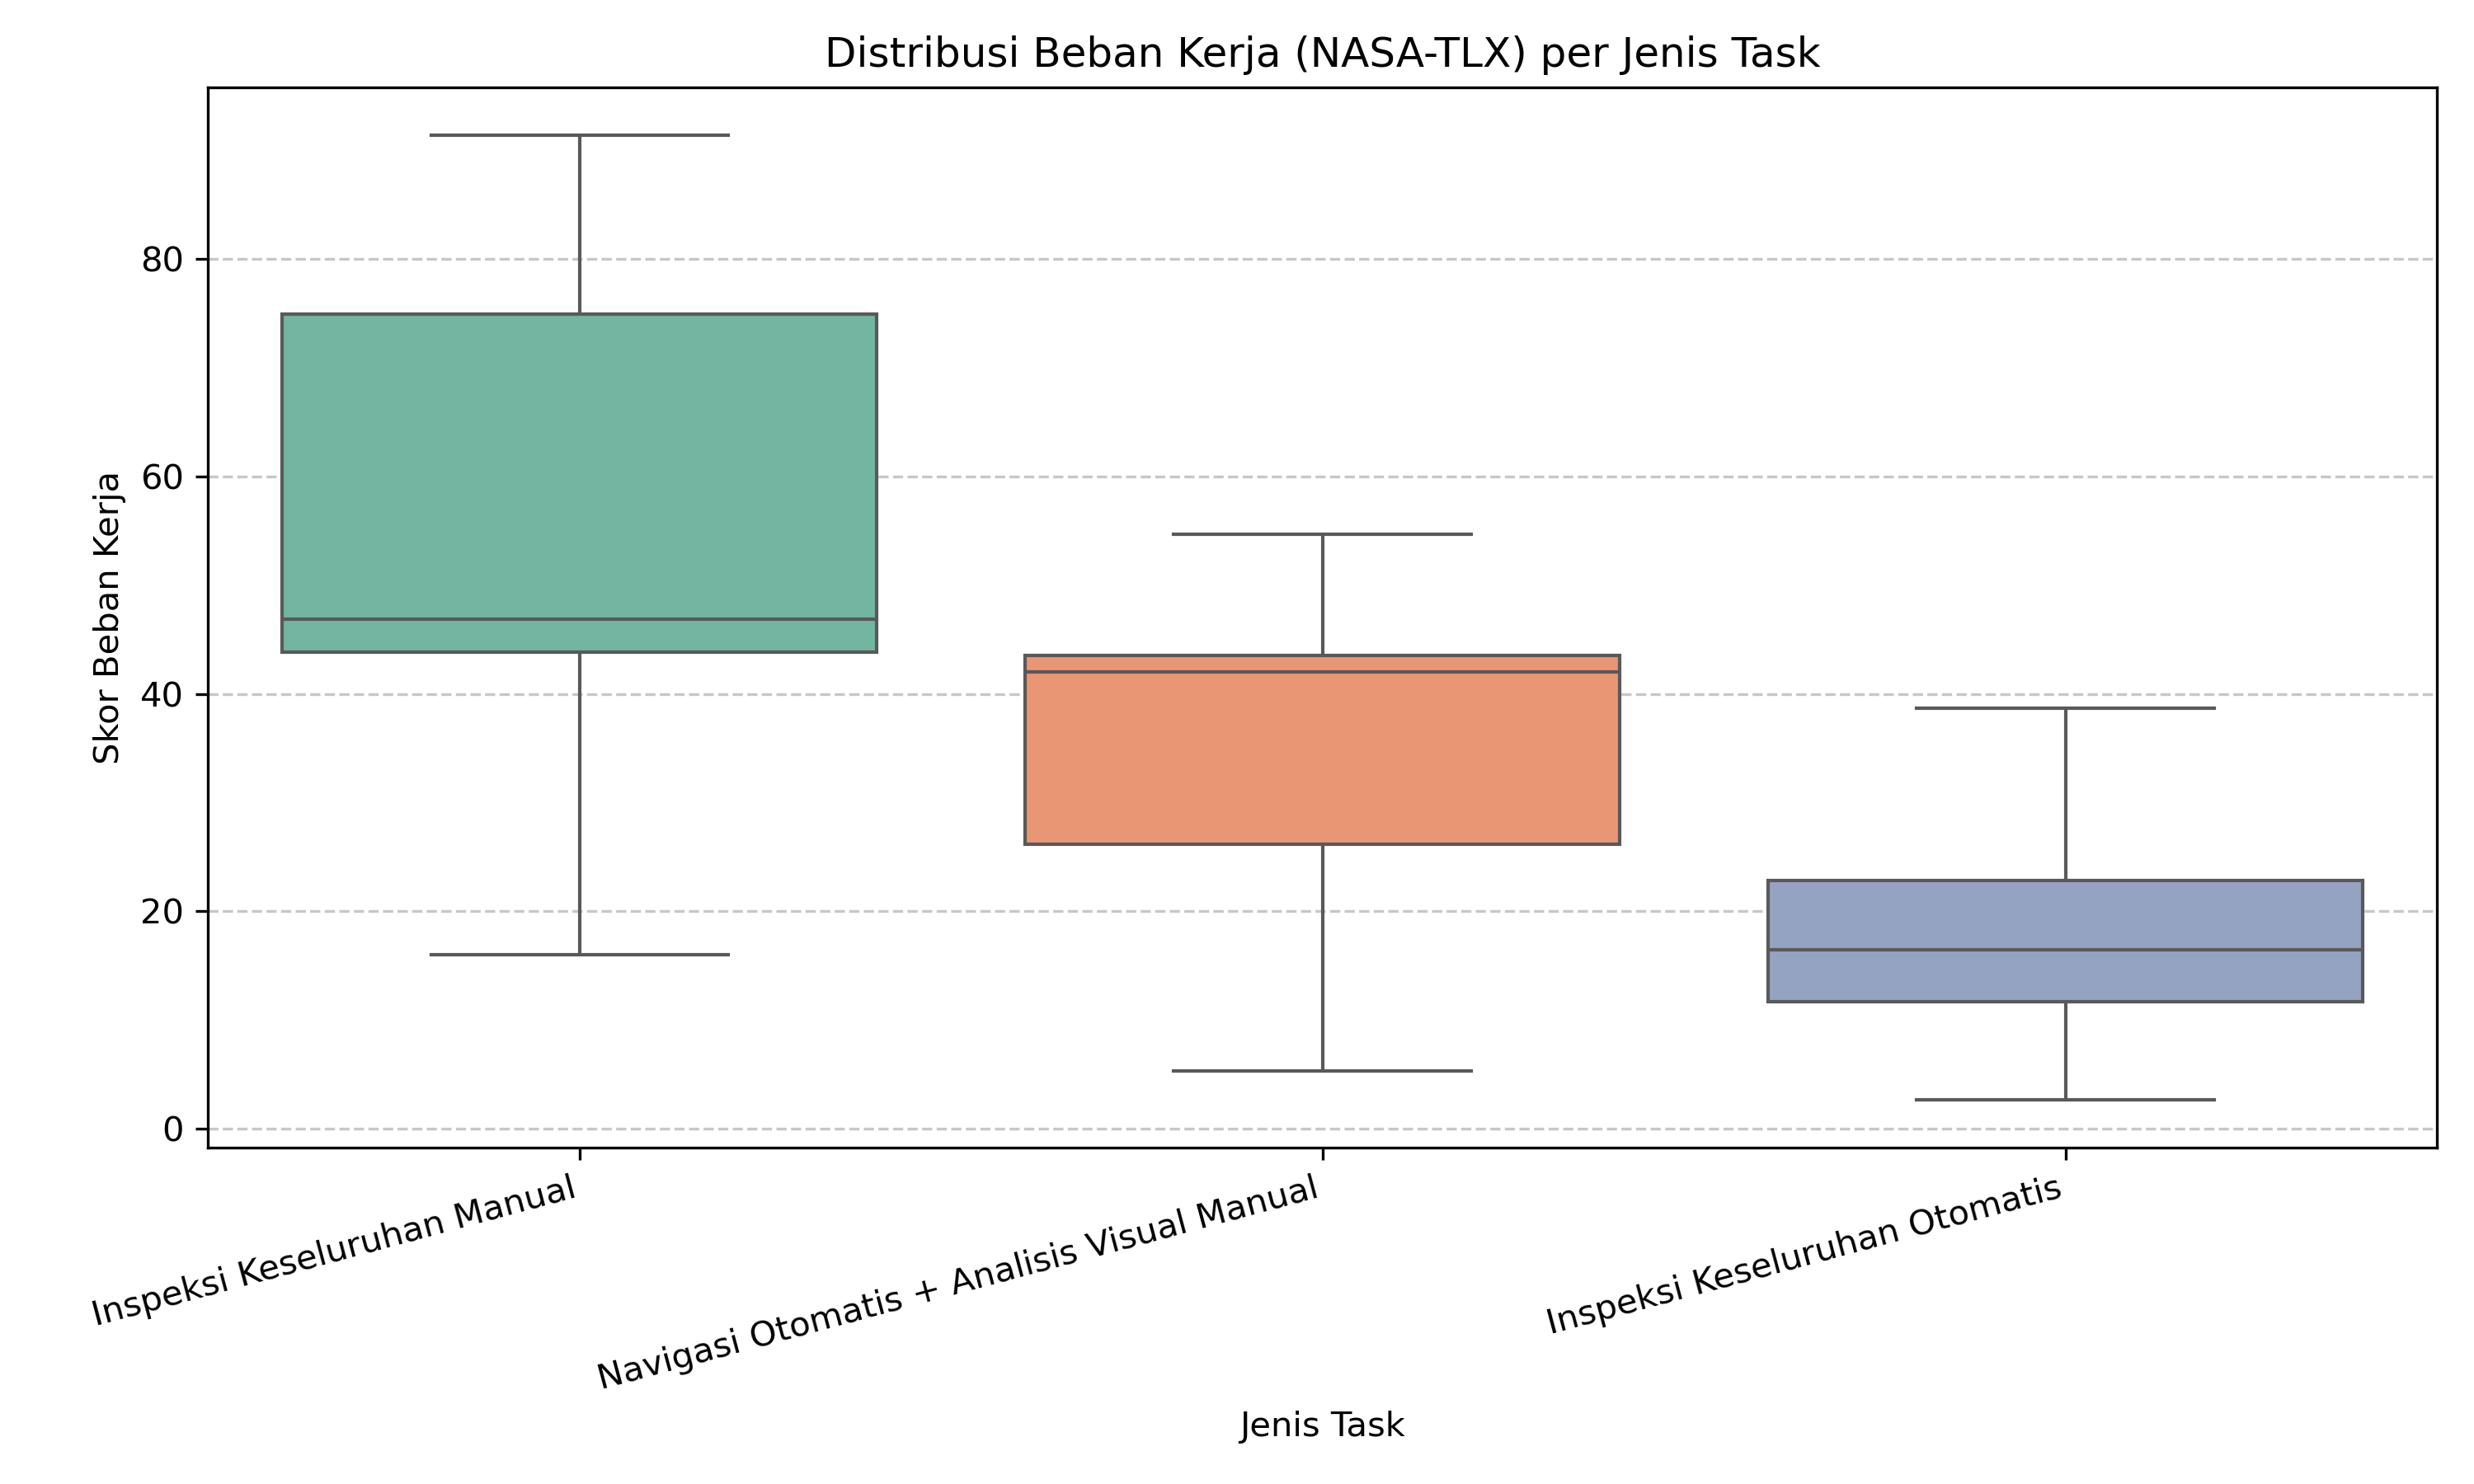
\includegraphics[width=0.8\textwidth]{Init/gambar/boxplots/boxplot_nasa_tlx.png}
    \caption{Distribusi Skor NASA-TLX untuk Tiga Kondisi Inspeksi}
    \label{fig:boxplot_nasa_tlx}
\footnotesize \textbf{Sumber:} Dokumentasi Penulis
\end{figure}

\subsection{Analisis Hasil}

Berdasarkan distribusi skor NASA-TLX yang divisualisasikan melalui \textit{boxplot} pada \textit{image} \ref{fig:boxplot_nasa_tlx} serta hasil pengujian yang disajikan pada Tabel \ref{tab:nasa_tlx_scores}, sistem inspeksi cerdas yang dikembangkan berhasil secara signifikan menurunkan beban kerja operator. Terlihat tren penurunan rata-rata skor beban kerja yang konsisten seiring dengan peningkatan level otonomi, dari 54,13 pada mode Inspeksi Keseluruhan Manual, turun menjadi 34,57 pada mode Navigasi Otomatis, dan mencapai titik terendah 18,40 pada mode Inspeksi Full Otomatis. Sistem ini berhasil menggeser kategori beban kerja operator dari level tinggi (\textit{High}) pada mode teleoperasi manual, menjadi level sedang (\textit{Medium}) saat robot menavigasi dirinya sendiri, hingga mencapai level rendah (\textit{Low}) ketika seluruh proses analisis visual juga diotomatisasi oleh MLLM.

Penurunan beban kerja secara umum bersumber pada reduksi tuntutan fisik dan mental. Pada mode manual, operator dituntut secara fisik untuk mengendalikan \textit{joystick} dan fokus menjaga kewaspadaan spasial dari kamera robot agar tidak menabrak halangan. Transisi ke navigasi otomatis mendelegasikan tugas gerak tersebut ke \textit{ROS Navigation Stack}, sehingga usaha fisik dan waktu yang dibutuhkan berkurang drastis. Selanjutnya, transisi ke mode full otomatis membebaskan operator dari kewajiban memproses dan mengklasifikasikan anomali objek secara kognitif, yang pada akhirnya meminimalisasi \textit{Mental Demand} dan \textit{Frustration Level}.

Kendati tren rata-rata secara keseluruhan menunjukkan penurunan beban kerja, analisis pada data individu mengungkap adanya beberapa anomali di mana beban kerja justru dirasakan meningkat pada mode otomatis. Anomali ini dipicu oleh dua faktor utama, yaitu faktor teknis dan psikologis. Dari segi teknis, kegagalan fungsi sistem saat uji coba lapangan, seperti disfungsi navigasi robot di lintasan atau kesalahan MLLM dalam menganalisis kondisi objek, secara langsung merusak persepsi kesuksesan misi. Kondisi ini mendorong operator untuk memberikan penalti skor yang berat pada dimensi Performansi (\textit{Performance}) dan Kebutuhan Waktu (\textit{Temporal Demand}). Sementara itu dari sisi psikologis, pergeseran peran dari pengendali aktif menjadi pengawas pasif pada tahap awal transisi otomatisasi sering kali memunculkan kecemasan. Operator yang belum sepenuhnya membangun rasa percaya terhadap sistem cenderung melakukan pengawasan berlebih. Hal ini justru membebani mereka secara mental dan menuntut usaha yang terkadang dirasa lebih melelahkan daripada mengendalikan robot secara langsung.

